% BEGIN PREAMBEL
\documentclass[9pt, xcolor=dvipsnames]{beamer}
\usepackage[british]{babel}
\usepackage{multimedia}
\usepackage{amsmath,amsfonts,amssymb}
\usepackage{upgreek}
\usepackage{pgfpages}
\usepackage[version=3]{mhchem}
\usepackage{lmodern}
\usepackage{graphicx}
\usepackage{multicol}
\usepackage{color}
\usepackage{xcolor,fontawesome,colortbl}
\usepackage{wrapfig}
\usepackage{siunitx}
\usepackage{fontspec}
\usepackage{tikz}
\usepackage{textpos}
\usepackage{booktabs}
\usepackage{caption}
\usepackage{subcaption}
\usepackage{wasysym}
\usepackage{animate}
\usepackage{tabularx}
\usepackage{ETHlogo}
\newfontfamily\ubuntu{Ubuntu}
\newcommand{\as}{\\[14pt]}
\newcommand{\s}{\\[7pt]}
\newcommand{\is}{\\[2pt]}
\newcommand{\no}{\noindent}
\newcommand{\ka}{\hspace*{0.5cm}}
\newcommand{\ma}{\hspace*{1cm}}
\newcommand{\ga}{\hspace*{1.5cm}}
\newcommand{\li}{\left|}
\newcommand{\re}{\right|}
\newcommand{\const}{\text{const.}}
\newcommand{\z}{\text}
\newcommand{\terminal}[1]{\colorbox{black}{\textcolor{white}{{\fontfamily{phv}\selectfont \scriptsize{#1}}}}}
\newcommand{\plugin}[1]{\textit{\flq#1\frq}}
\newcommand{\ra}{$\rightarrow$ }
\definecolor{cadmiumgreen}{rgb}{0.0, 0.42, 0.24}
\newcommand{\itemfill}{\setlength{\itemsep}{\fill}}
\newcommand{\orderof}[1]{$\mathcal{O}\left(#1\right)$}
\newcommand{\good}[1]{\usebeamercolor[fg]{title} \textbf{#1}}

\usetheme{Boadilla}
\graphicspath{ {Pics/} }
\makeatletter
\def\input@path{ {sections/} }
\makeatother
\usecolortheme[named=ForestGreen]{structure}
\useoutertheme{miniframes}
\sisetup{detect-weight=true, detect-family=true}
\beamertemplatenavigationsymbolsempty
\makeindex
\author[M. Reichmann]{Michael Reichmann}
\institute[\textbf{\textit{ETH}}\scalebox{.6}{\textit{Z\"{u}rich}}]{Swiss Federal Institute of Technology Zurich}
\AtBeginSection{\frame[noframenumbering]{\sectionpage}}

\setbeamercolor{frametitle}{bg=date in head/foot.bg!20!white}

%% TITLE PAGE
\defbeamertemplate*{title page}{customized}[1][] {
	\ETHlogo[3cm]
	\vspace*{-33pt}
	\begin{figure}[t]
		\flushright
		
\includegraphics[height=.9cm]{IPP}
	\end{figure}
	\vspace*{-10pt}
	\begin{figure}
		\centering
		\includegraphics[width=.6\textheight]{\inserttitlegraphic}
	\end{figure}
	\begin{block}{}
		\centering
		\vspace*{1pt}
		\usebeamerfont{title}\usebeamercolor[fg]{title}\textbf{\inserttitle}\\\vspace*{5pt}
		\usebeamerfont{subtitle}\insertsubtitle\\\vspace*{1pt}
	\end{block}
	\vspace*{10pt}
	\centering
	\color{black}
	\usebeamerfont{author}\textbf{\insertauthor}\par\vspace*{2pt}
	\usebeamerfont{author}on behalf of the RD42 Collaboration\par\vspace*{5pt}
	\usebeamerfont{date}\insertdate\par
}

%% FOOTLINE
\setbeamertemplate{footline}
{
  \leavevmode%
  \hbox{%
  \begin{beamercolorbox}[wd=.3\paperwidth,ht=2.25ex,dp=1ex,center]{author in head/foot}%
    \usebeamerfont{author in head/foot}\insertshortauthor\hspace*{2pt}
    (
\includegraphics[height=3.5pt]{ETHLogoWhite})
  \end{beamercolorbox}%
  \begin{beamercolorbox}[wd=.4\paperwidth,ht=2.25ex,dp=1ex,center]{title in head/foot}%
    \usebeamerfont{title in head/foot}\insertshorttitle
  \end{beamercolorbox}%
  \begin{beamercolorbox}[wd=.3\paperwidth,ht=2.25ex,dp=1ex,right]{date in head/foot}%
    \usebeamerfont{date in head/foot}\insertdate\hspace*{3em}
    \insertframenumber{} / \inserttotalframenumber\hspace*{1ex}
  \end{beamercolorbox}}%
  \vskip0pt%
}
 
%% SECTION PAGE
\setbeamertemplate{section page}
{
    \begin{centering}
		\usebeamerfont{title}Section \insertsectionnumber\\\vspace*{.7cm}
		\begin{beamerboxesrounded}[shadow=true, lower=frametitle]{}
			\centering
			\vspace*{3pt}
			\usebeamerfont{frametitle}\textbf{\insertsection}\par
			\vspace*{3pt}
		\end{beamerboxesrounded}
    \end{centering}
}

\title[Diamond Detectors]{Diamond Detector Technology: Status and Perspectives}
\subtitle{EPS Conference (Venice, Italy)}
\titlegraphic{RocFull}
\date{7th July 2017}
% END PREAMBEL

\begin{document}

% ============= TITLE PAGE =============
\usebackgroundtemplate{\tikz\node[opacity=0.2] {\hspace*{-5pt}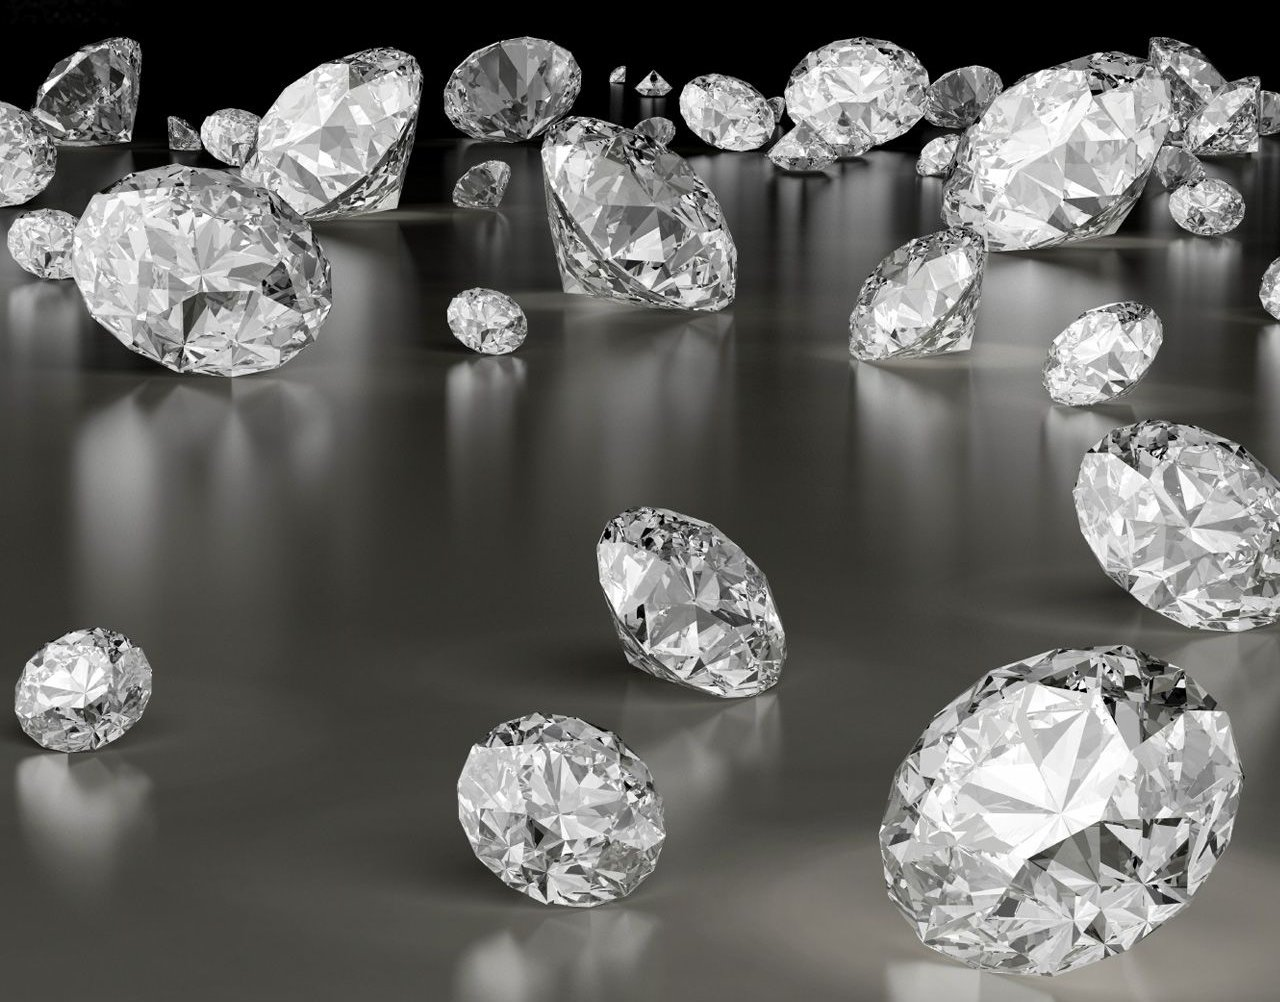
\includegraphics[height=\paperheight,width=1.05\paperwidth]{bkg.jpg}};}
\maketitle
\usebackgroundtemplate{}

% ============= TABLE OF CONTENTS ======
\begin{frame}%[allowframebreaks]
	\frametitle{Table of contents}
	\tableofcontents[hideallsubsections]   % [pausesections]
\end{frame}

% ============= 1 =============
% \section{}
% \include{}

% ============= 1 =============
\section{Motivation}
\begin{frame}{Motivation}

	\begin{itemize}
		\item innermost layers \ra highest radiation damage (\SIrange{100}{200}{\mega\hertz\per cm^2})
		\item current detector is designed to survive \SI{\sim12}{month} in High-Luminosity LHC
		\item \usebeamercolor[fg]{title} \textbf{\ra R\&D for more radiation hard detector designs and/or materials}
	\end{itemize}\vspace*{10pt}
	
	\uncover<2->{
		\textbf{\underline{Diamond as Detector Material:}}\vspace*{5pt}
		\begin{itemize}
			\itemfill
			\item properties 
			\begin{itemize}
				\itemfill
				\item radiation tolerance
				\item isolating material
				\item high charge carrier mobility
				\item \textcolor{RedOrange}{smaller signal than in silicon}
			\end{itemize}
		\end{itemize}}

% 	\uncover<3->{
% 		\begin{itemize}
% 			\item diamond pixel detectors in Pixel Luminosity Telescope (PLT) (installed 2010/2011)
% 			\begin{itemize}
% 				\item \textcolor{RedOrange}{\textbf{signal dependence on incident particle rate observed}} (single crystal)
% 			\end{itemize}
% 		\end{itemize}}
	
	\uncover<3->{
		\begin{itemize}
			\item investigation of the signal independence/dependence on incident particle flux in various detector designs:
			\begin{itemize}
				\itemfill
				\item pad \ra full diamond as single cell readout
				\item pixel \ra diamond sensor on pixel chips
				\item 3D \ra strip/pixel detector with clever design to reduce drift distance
			\end{itemize}

		\end{itemize}}
		
\end{frame}


% ============= 2 =============
\section{Diamond Types}
\begin{frame}{Diamond Types}

	\begin{itemize}
		\itemfill
		\item diamonds artificially grown with chemical vapour deposition (CVD)
		\item investigation of two different diamond types:
	\end{itemize}
	
	\begin{figure}[h] 
		\centering
		\begin{subfigure}{0.45\textwidth}  
			\centering
			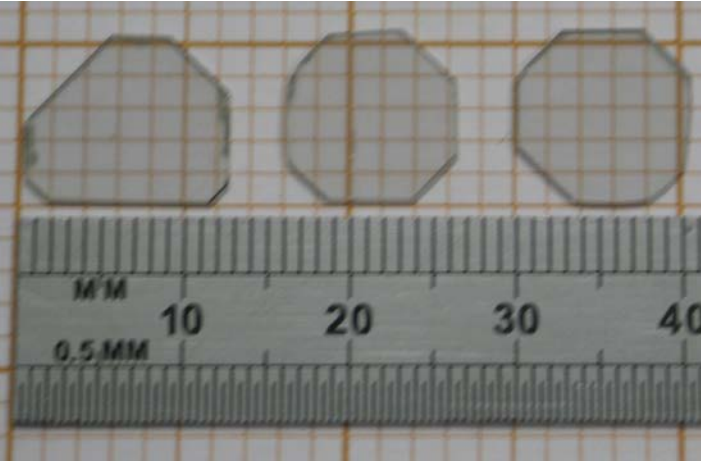
\includegraphics[height=0.4\textheight]{scDia}
			\caption{single-crystalline CVD}
		\end{subfigure}
		\begin{subfigure}{0.45\textwidth} 
			\centering
			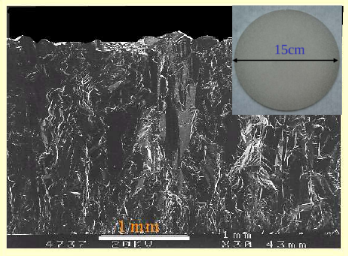
\includegraphics[height=0.4\textheight]{pCVD1}
			\caption{poly-crystalline CVD (courtesy of E6)} 	
		\end{subfigure} 
	\end{figure}\vspace*{-5pt}
	
	\hspace*{10pt}
	\begin{minipage}{5.5cm}
		\begin{itemize}
% 			\item grown on existing diamond crystal
			\item only small sizes (\SI{\sim.25}{cm^2})
% 			\item larger signals than pCVD ($5:3$)
%  			\item full charge collection
		\end{itemize}
	\end{minipage}
	\hspace*{2pt}
	\begin{minipage}{5.5cm}
		\begin{itemize}
% 			\item grown on Si substrate with diamond powder
			\item large wafers (\SIrange{5}{6}{''} \diameter)
% 			\item non-uniformities and grains
% 			\item collection distance up to \SI{500}{\micro\meter}
		\end{itemize}
	\end{minipage}
	
	\begin{itemize}
		\item pCVD signals smaller than scCVD (1:2) in planar configuration
	\end{itemize}

	
\end{frame}


% ============= 3 =============
\section{Radiation Tolerance}
\subsection{Setup}
% ============================ FRAME 1 ============================================
\begin{frame}{Devices}

	\begin{figure}[h] 
		\centering
		\begin{subfigure}{0.45\textwidth}  
			\centering
			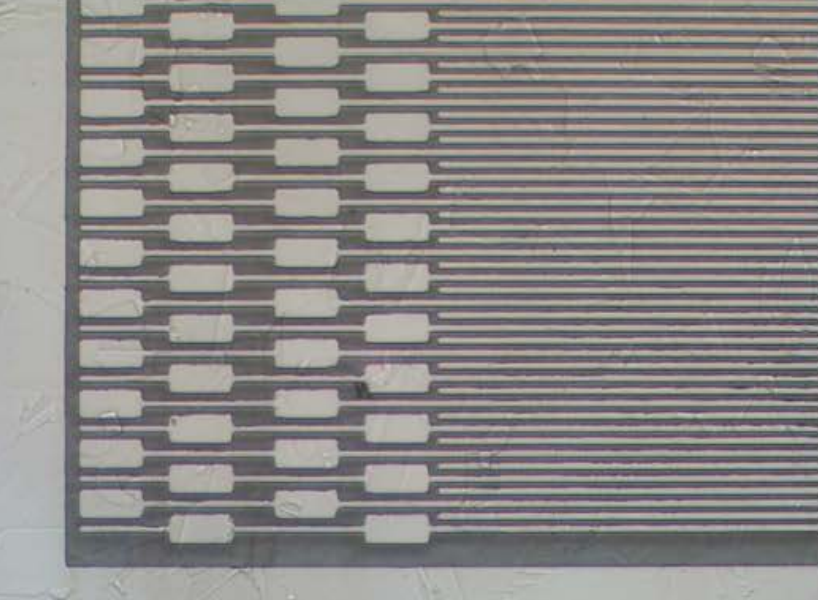
\includegraphics[height=0.4\textheight]{RadMetal}
			\caption{strip metalisation pattern}
		\end{subfigure}
		\begin{subfigure}{0.45\textwidth} 
			\centering
			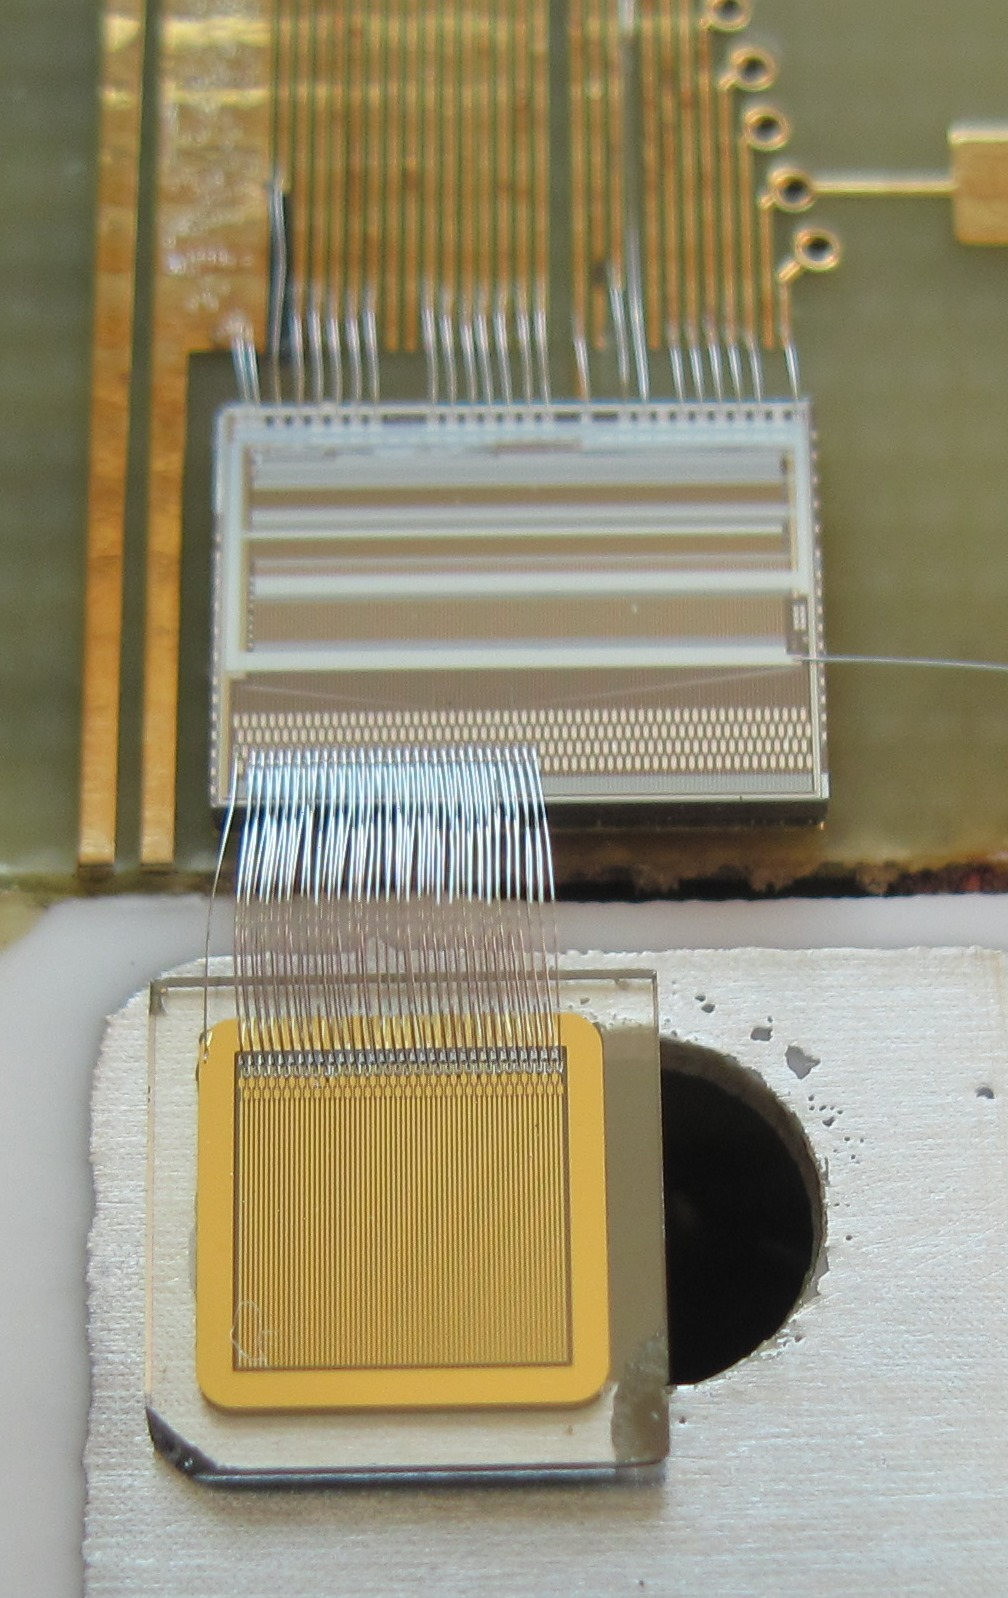
\includegraphics[width=0.4\textheight, angle=-90]{StripVA}
			\caption{mounted diamond with amplifier} 	
		\end{subfigure} 
	\end{figure}
	
	\begin{itemize}
		\itemfill
		\item patterning the diamonds \ra create pad, strip and pixel devices
		\item metalisation on both sides \ra almost edgeless 
		\item segmentation critical for radiation studies \ra charge \& position
	\end{itemize}

\end{frame}
% ============================ FRAME 2 ============================================
\begin{frame}{Schematic Beam Test Setup}

	\begin{figure}[h] 
		\centering
		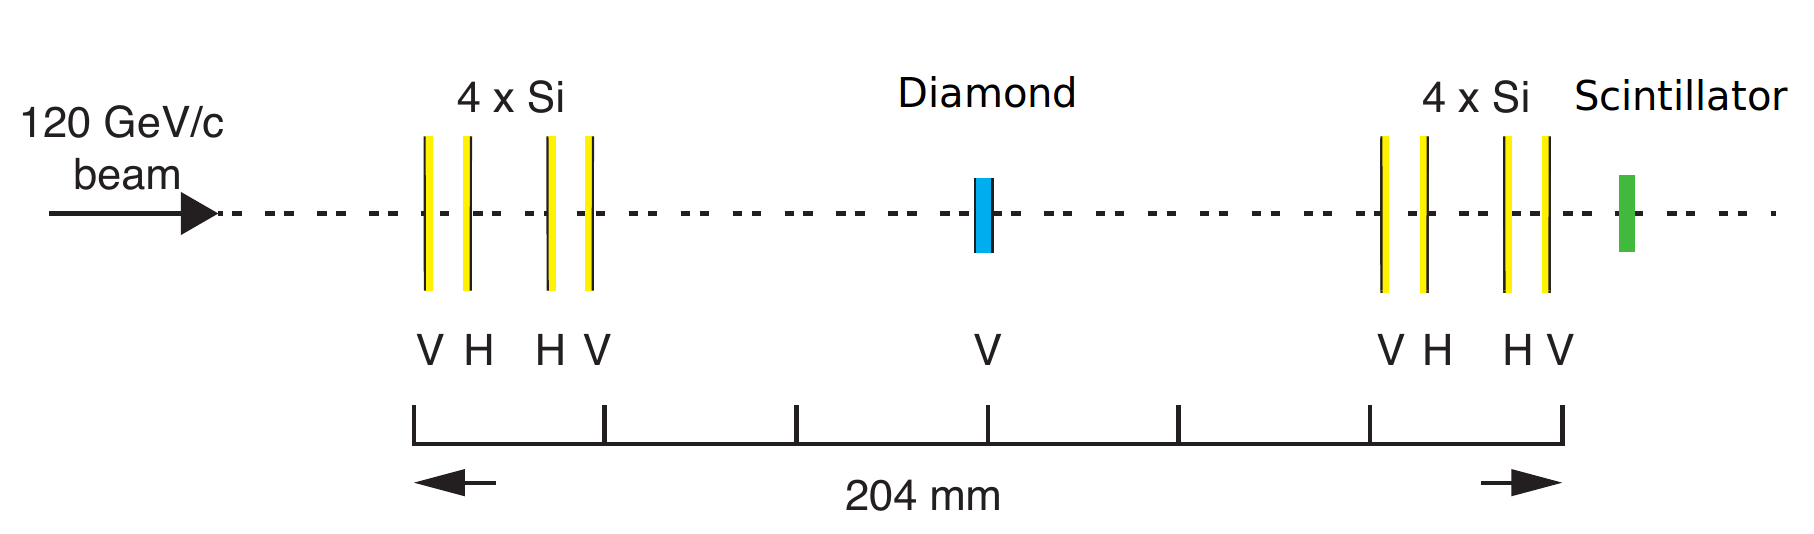
\includegraphics[width=\textwidth]{RadTel}
	\end{figure}
	
	\begin{itemize}
		\itemfill
		\item characterisation of irradiated devices in beam tests
		\item transparent or unbiased hit predictions from telescope
	\end{itemize}

\end{frame}

\subsection{Results}
% ============================ FRAME 3 ============================================
\begin{frame}{Irradiation at CERN PS with \SI{24}{\giga\electronvolt} protons}

	\begin{minipage}{4.5cm}
		\underline{damage equation:}
		\vspace*{-3pt}
		\begin{align*}
			\z{n} 				&= \z{n}_0 + \z{k}\upphi\\
			\frac{1}{\z{mfp}}	&= \frac{1}{\z{mfp}_0} + \z{k}\upphi
		\end{align*}
		\vspace*{-5pt}
		\begin{itemize}
			\item[\textcolor{black}{$\z{n}_0$}] $-$ initial number of traps
			\item[\textcolor{black}{$\z{mfp}_0$}] $-$ initial mean free path
			\item[\textcolor{black}{k}] $-$ damage constant
			\item[\textcolor{black}{$\upphi$}] $-$ fluence
		\end{itemize}
	\end{minipage}
	\hspace*{2pt}
	\begin{minipage}{6.5cm}
		\begin{figure}[h]
			\centering
			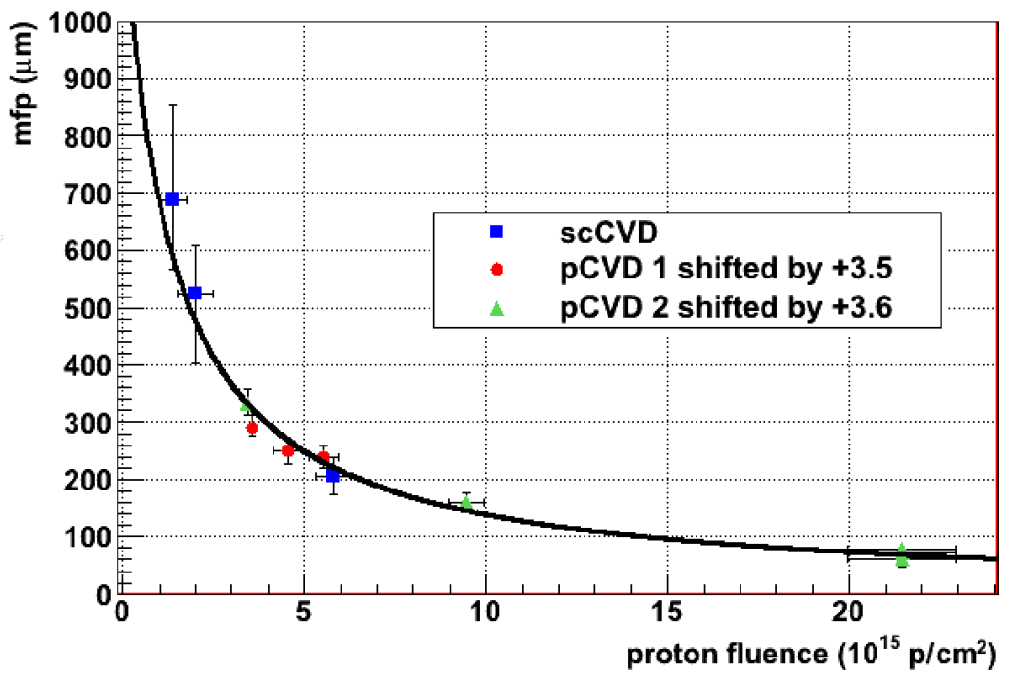
\includegraphics[width=6.5cm]{Damage24}
		\end{figure}
	\end{minipage}
	
	\begin{itemize}
		\itemfill
		\item assume same mean free path for electrons and holes
		\item results up to \SI{2.2e16}{p\per cm^2} (\SI{\sim500}{\mega rad})
		\item same damage curves and constant (k) for scCVD and pCVD diamonds
		\item larger $\z{mfp}_0$ performs better at any fluence 
	\end{itemize}

\end{frame}
% ============================ FRAME 4 ============================================
\begin{frame}{Charge Collection Distance (ccd) vs. Mean Free Path (mfp)}
	
	\begin{itemize}
		\itemfill
		\item ccd = average distance between electron and hole until trapped
		\item for scCVD: ccd $\sim$ thickness, for pCVD: ccd < thickness
% 		\item ccd coincides with mfp for mfp $\ll$ thickness
		\item ccd direct measurement (no correction)
		\item mfp correct theory \ra correct data with assumptions (i.\,a. $\z{mfp}_{\z{e}}=\z{mfp}_{\z{h}}$)
	\end{itemize}
	
	\begin{minipage}{6cm}
		\underline{equation for ccd:}
		\vspace*{-3pt}
		\begin{equation*}
			\frac{\z{ccd}}{\z{t}} = \sum_i \frac{\z{mfp}_i}{\z{t}}\left(1-\frac{\z{mfp}_i}{\z{t}}\left(1-\z{e}^{-\frac{\z{t}}{\z{mfp}_i}}\right)\right)
		\end{equation*}
		\vspace*{-5pt}
		\begin{itemize}
			\item[\textcolor{black}{t}] $-$ thickness
			\item[\textcolor{black}{$i$}] $-$ electrons \& holes
		\end{itemize}
	\end{minipage}
	\hspace*{2pt}
	\begin{minipage}{5cm}
		\begin{figure}[h]
			\centering
			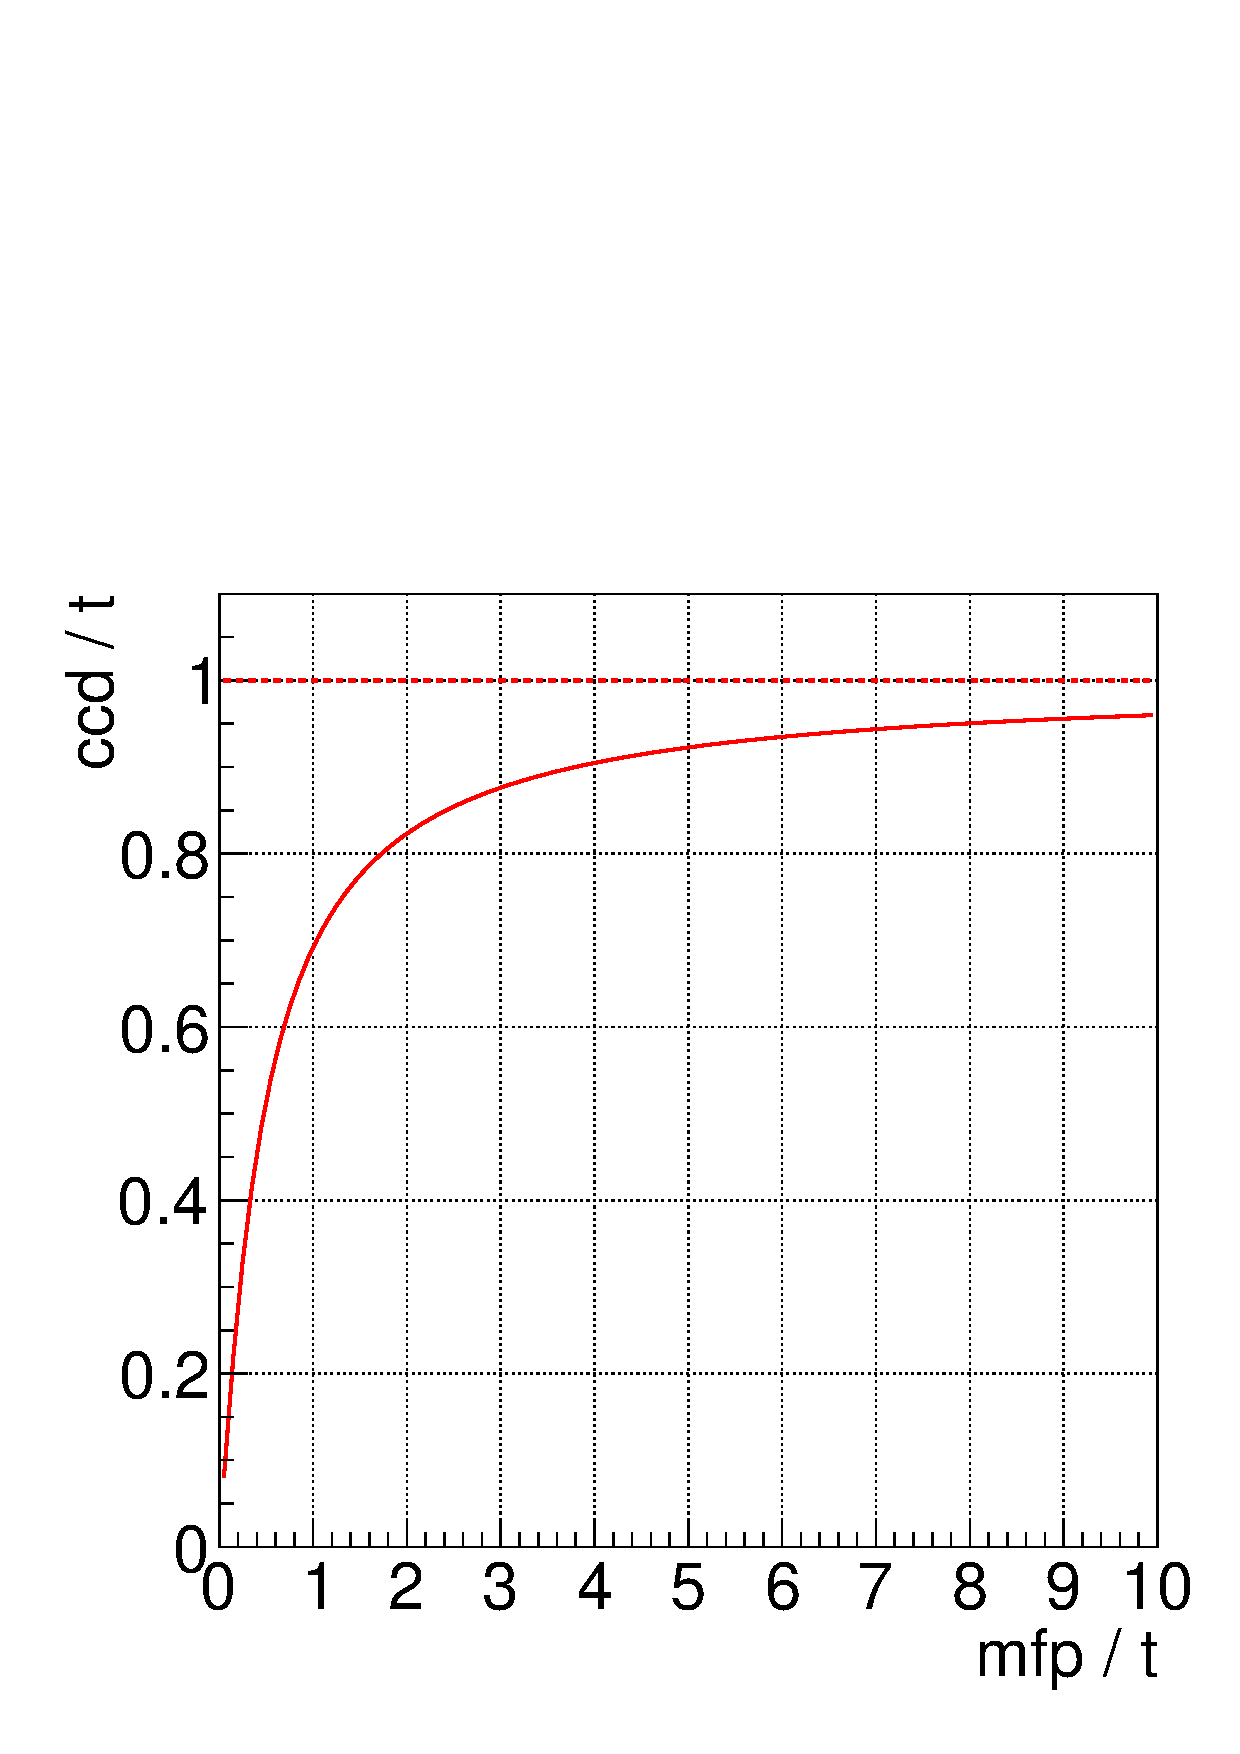
\includegraphics[width=4.5cm]{CCDMFP}
		\end{figure}
	\end{minipage}

\end{frame}
% ============================ FRAME 5 ============================================
% \begin{frame}{Irradiation at LANL with \SI{800}{\mega\electronvolt} protons}
% 
% 	\begin{figure}[h] 
% 		\centering
% 		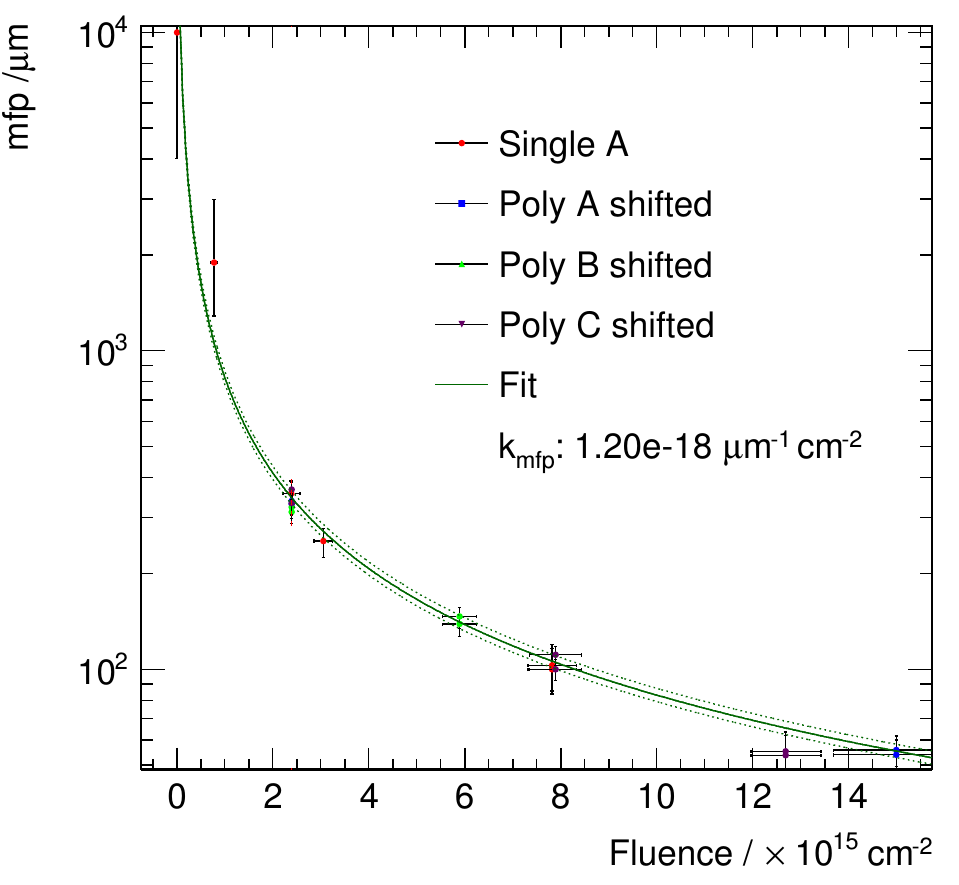
\includegraphics[width=.3\textwidth]{Damage800}
% 	\end{figure}
% 	
% 	\begin{itemize}
% 		\itemfill
% 		\item irradiation results up to \SI{1.4e16}{p\per cm^2}
% 		\item same damage curve:
% 	\end{itemize}
% 	\vspace*{-5pt}
% 	\begin{equation*}
% 		\frac{1}{\z{mfp}} = \frac{1}{\z{mfp}_0} + \z{k}\upphi
% 	\end{equation*}
% 	\vspace*{-5pt}
% 	\begin{itemize}
% 		\item \SI{800}{\mega\electronvolt} protons \SIrange{1.6}{1.8}{} more damaging than \SI{24}{\giga\electronvolt} protons
% 	\end{itemize}
% 
% \end{frame}
% ============================ FRAME 6 ============================================
\begin{frame}{Summary of Proton, Neutron and Pion Irradiation}

	\begin{figure}[h] 
		\centering
		\begin{subfigure}{0.45\textwidth}  
			\centering
			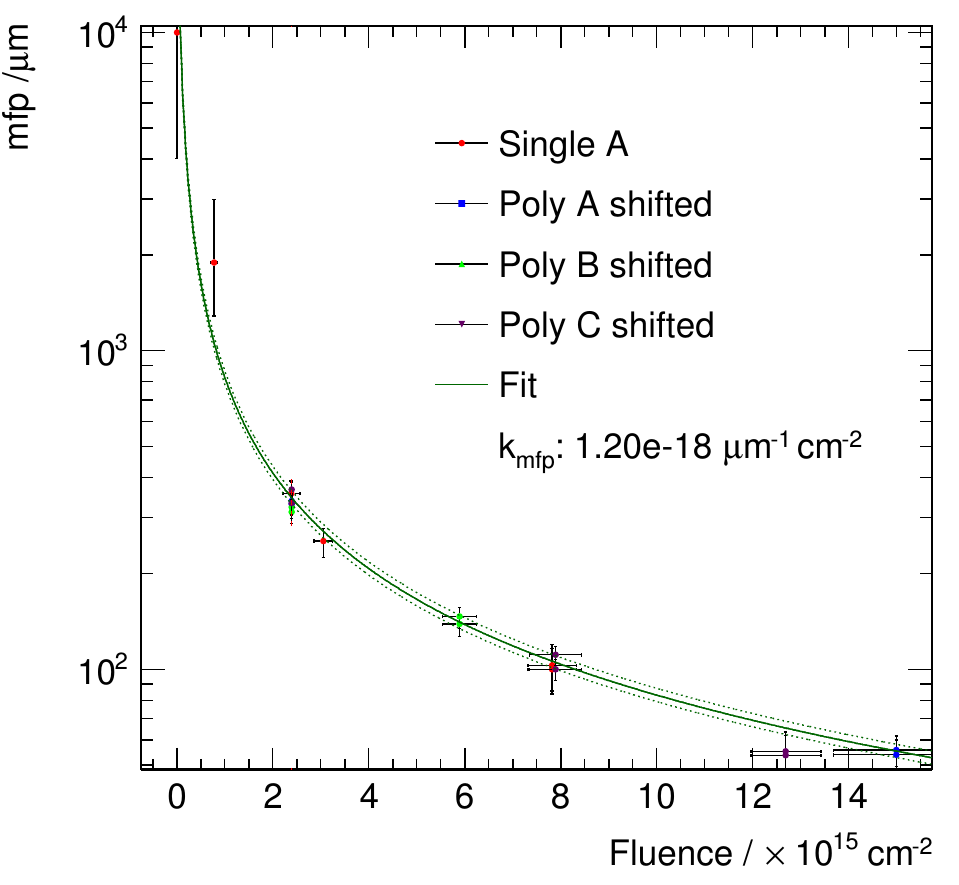
\includegraphics[height=0.5\textheight]{Damage800}
			\caption{irradiation at LANL with \SI{800}{\mega\electronvolt} protons (up to \SI{1.4e16}{p\per cm^2})}
		\end{subfigure}
		\begin{subfigure}{0.45\textwidth} 
			\centering
			\vspace*{25pt}
			\begin{tabular}[c]{l|l|l}
				\noalign{\hrule height 1pt}
				\rowcolor{title in head/foot.bg!70!white} 
	% 			\rowcolor{author in head/foot.bg} 
	% 			\rowcolor{date in head/foot.bg} 
				\multicolumn{1}{c|}{\textbf{Particle}} & \multicolumn{1}{c|}{\textbf{Energy}} & \multicolumn{1}{c}{\textbf{Relative k}} \\\hline
				\rowcolor{date in head/foot.bg!30!white} 
				Proton 	& \SI{24}{\giga\electronvolt} 	& $1.0$ 			\\\hline
						& \SI{800}{\mega\electronvolt} 	& $1.79 \pm 0.13$ 	\\\hline
				\rowcolor{date in head/foot.bg!30!white} 
						& \SI{70}{\mega\electronvolt} 	& $2.4 	\pm 0.4$ 	\\\hline
						& \SI{25}{\mega\electronvolt} 	& $4.5 	\pm 0.6$ 	\\\hline
				\rowcolor{date in head/foot.bg!30!white} 
				Neutron	& \SI{1}{\mega\electronvolt} 	& $4.5 	\pm 0.5$ 	\\\hline
				Pion	& \SI{200}{\mega\electronvolt} 	& $2.5 	- 3$ 		\\
				\noalign{\hrule height 1pt}
			\end{tabular}
			\caption{summary}
		\end{subfigure}
	\end{figure}
	
% 	\begin{itemize}
% 		\item data fits displacement energy (DPA) better than non ionising energy loss (NIEL) theories
% 		\item DPA need to be tuned to diamonds
% 	\end{itemize}

\end{frame}


% ============= 4 =============
\section{Diamond Devices in Experiments}
\begin{frame}{Diamond Devices in Experiments}

	\begin{itemize}
		\itemfill
		\item beam condition/loss monitors
		\begin{itemize}
			\item essential in all modern collider experiments
		\end{itemize}
		\item current generation pixel detectors
		\begin{itemize}
			\item \good{ATLAS Diamond Beam Monitor (DBM)}
		\end{itemize}
		\item future HL-LHC trackers
		\begin{itemize}
			\item \good{3D diamond detectors}
		\end{itemize}
		\item future beam condition/luminosity monitor
		\begin{itemize}
			\item multipad design BCM'
		\end{itemize}
	\end{itemize}\vspace*{10pt}
		
\end{frame}

\subsection{ATLAS DBM}
% ============================ FRAME 2 ============================================
\begin{frame}{ATLAS DBM}

	\vspace*{-5pt}
	\begin{itemize}
		\itemfill
		\item diamond pixel detectors in ATLAS (tracking)
		\item total production of 45 diamonds (t $=$ \SI{500}{\micro\meter}) on FE-I4b chips
		\item module assembly at CERN
		\item installed during LS1
		\item 8 telescopes (2 Si \& 6 Diamond) symmetric around ATLAS IP
% 		\item \SI{854}{\milli\meter} < |z| < \SI{1092}{\milli\meter}, 3.2 < |$\upeta$| < 3.5
		\item thresholds tuned to \SI{\sim 2500}{e}
	\end{itemize}
	\vspace*{-5pt}

	\begin{figure}[h] 
		\centering
		\begin{subfigure}{0.45\textwidth}  
			\centering
			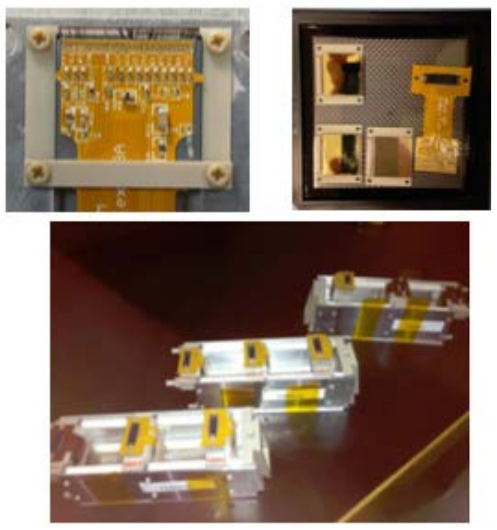
\includegraphics[height=0.38\textheight]{DBM2}
			\caption{cable, detectors, telescopes}
		\end{subfigure}
		\begin{subfigure}{0.45\textwidth} 
			\centering
			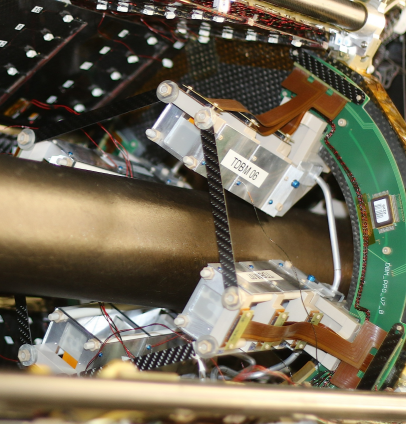
\includegraphics[height=0.38\textheight]{DBM1}
			\caption{4 mounted telescopes } 	
		\end{subfigure} 
	\end{figure}\vspace*{-15pt}

\end{frame}
% ============================ FRAME 3 ============================================
% \begin{frame}{Thresholds}
% 
% 	\begin{itemize}
% 		\itemfill
% 		\item ATLAS DBM integrated in ATLAS readout in 2015
% 		\item thresholds tuned to \SI{2500}{e}
% 	\end{itemize}
% 
% 	\vspace*{-5pt}
% 	\begin{figure}[h] 
% 		\centering
% 		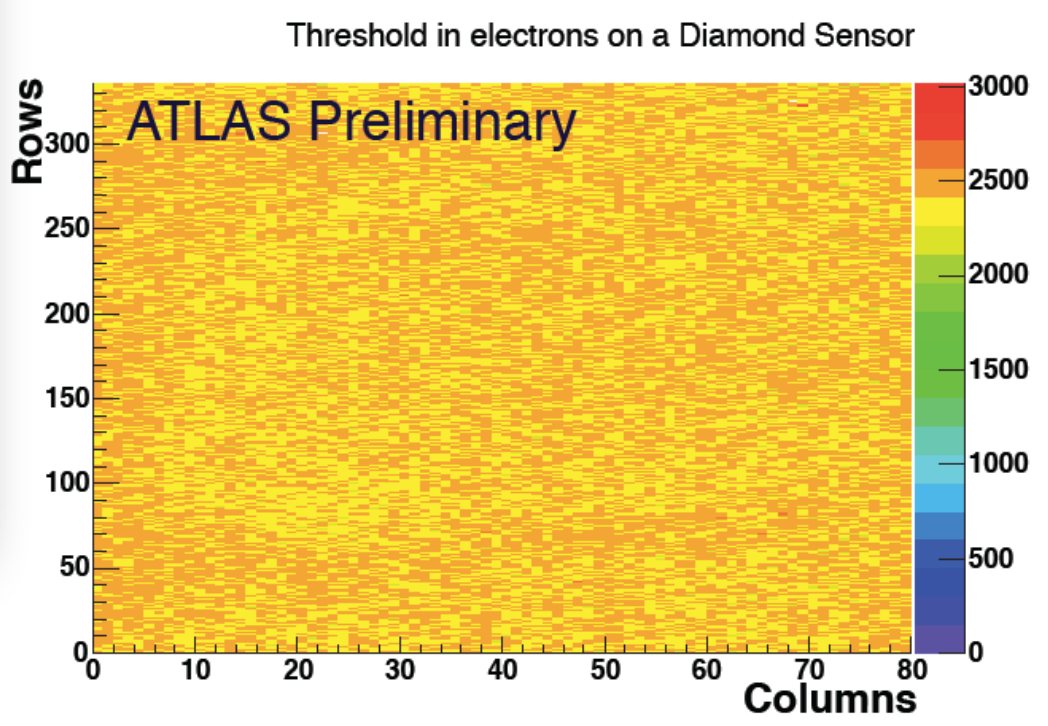
\includegraphics[height=0.5\textheight]{DBMThresh}
% 	\end{figure}
% 	\vspace*{-5pt}
% 
% 	\begin{itemize}
% 		\itemfill
% 		\item lower threshold as much as possible (\SI{\sim1100}{e} achieved on bench)
% 		\item operation issues during data taking
% 	\end{itemize}
% 
% \end{frame}
% ============================ FRAME 4 ============================================
\begin{frame}{Tracking}

	\begin{itemize}
		\itemfill
		\item reconstruction of tracks from hits of 3 modules
	\end{itemize}

	\vspace*{-5pt}
	\begin{figure}[h] 
		\centering
		\begin{subfigure}{0.4\textwidth}  
			\centering
			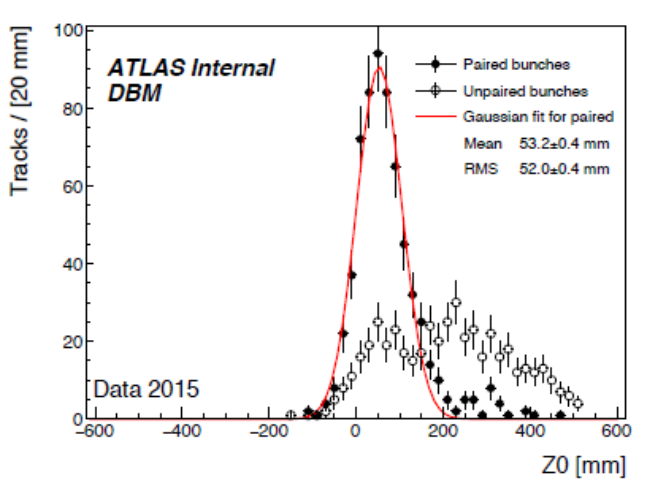
\includegraphics[height=0.4\textheight]{DBMTrack1}
			\caption{longitudinal distance to IP}
		\end{subfigure}
		\begin{subfigure}{0.18\textwidth} 
			\centering
			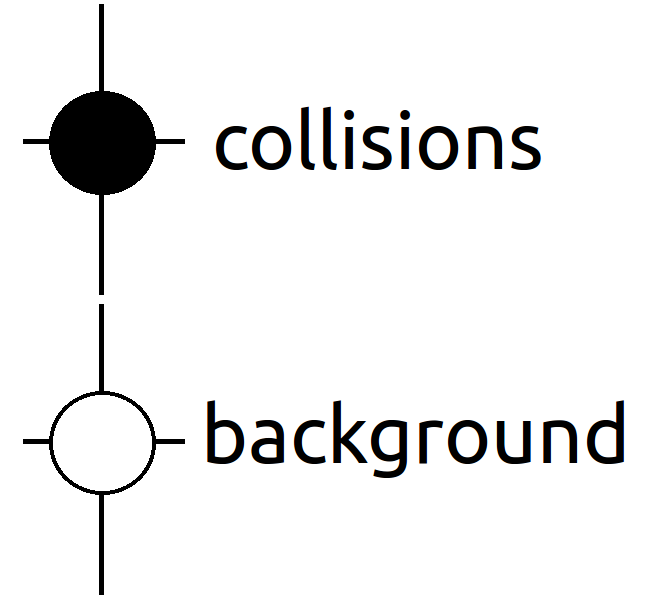
\includegraphics[height=0.2\textheight]{DBMLegend}
		\end{subfigure} 
		\begin{subfigure}{0.4\textwidth} 
			\centering
			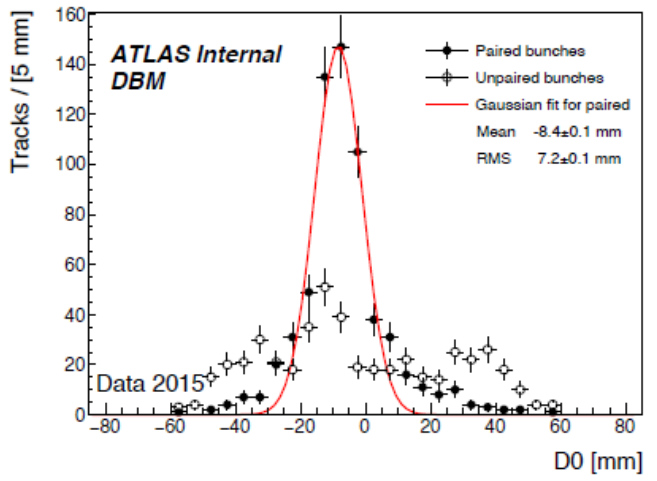
\includegraphics[height=0.4\textheight]{DBMTrack2}
			\caption{radial distance to IP} 	
		\end{subfigure}
	\end{figure}
	\vspace*{-10pt}

	\begin{itemize}
		\itemfill
		\item plots with initial alignment
		\item clear discrimination between background and collisions
		\item loss of modules (Si/D)
			\begin{itemize}
				\item successful re-commissioning of surviving modules
			\end{itemize}
		\item diamond and Si modules now part of ATLAS data taking
	\end{itemize}

\end{frame}

% ============= 5 =============
\section{Rate Studies}
\subsection{pCVD Diamond Pad Detectors}
\begin{frame}{Setup}
	
	\begin{itemize}
		\itemfill
		\item rate studies conducted with \SI{260}{\mega\electronvolt\per c} $\uppi^+$ at Paul Scherrer Institute (PSI)
		\item tunable particle fluxes from \orderof{\SI{1}{\kilo\hertz\per cm^2}} to \orderof{\SI{10}{\mega\hertz\per cm^2}}
		\item detectors tested in ETHZ beam telescope (based on CMS-Pixel-Chips)
	\end{itemize}

	\vspace*{-5pt}
	\begin{figure}[h] 
		\centering
		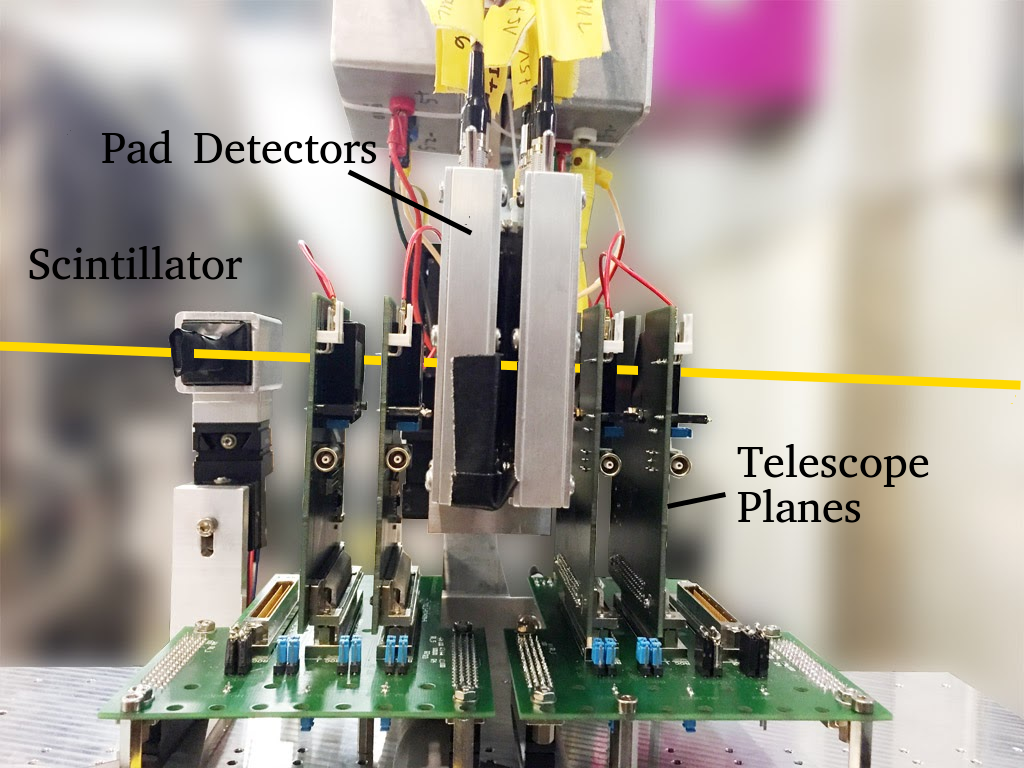
\includegraphics[height=.4\textheight]{Setup}
	\end{figure}
	\vspace*{-5pt}
	
	\begin{itemize}
		\item 4 tracking planes with particle trigger
		\item scintillator for precise trigger timing \ra \orderof{\SI{1}{\nano\second}}
	\end{itemize}

\end{frame}

% ============================ FRAME 2 ============================================
\begin{frame}{Pad Detectors}

	\begin{figure}[h] 
		\centering
		\begin{subfigure}{0.45\textwidth}  
			\centering
			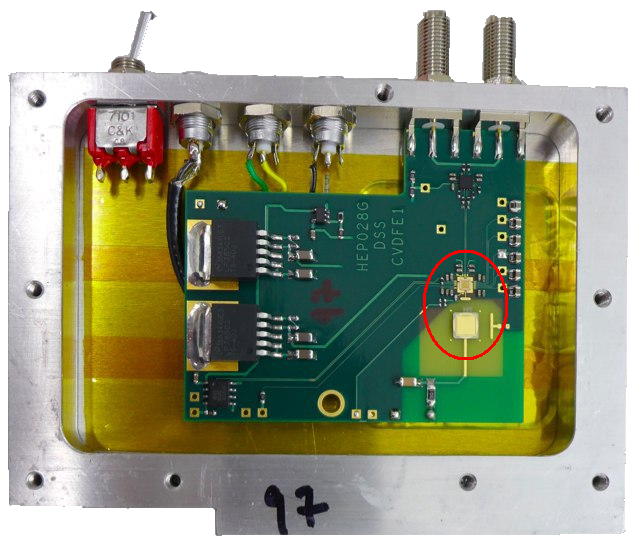
\includegraphics[height=0.45\textheight]{PadBox}
			\caption{fast amplifier box}
		\end{subfigure}
		\begin{subfigure}{0.45\textwidth} 
			\centering
			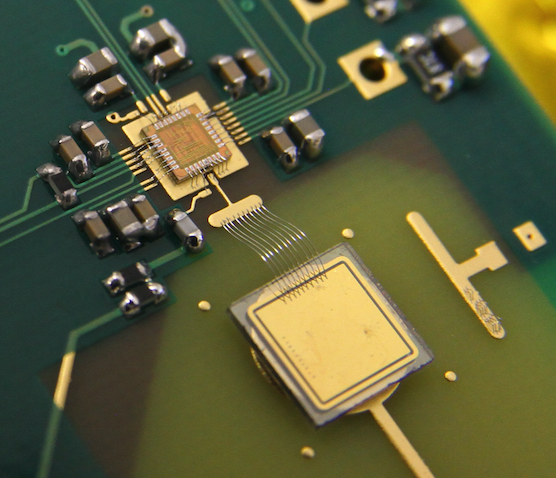
\includegraphics[height=0.45\textheight]{PadFull}
			\caption{diamond and fast amp} 	
		\end{subfigure} 
	\end{figure}
	\vspace*{-10pt}
	
	\begin{itemize}
		\itemfill
		\item diamonds in custom built amplifier boxes from Ohio State University (OSU)
		\item cleaning, photo-lithography and Cr-Au metallisation at OSU
		\item low noise, fast amplifier with \orderof{\z{5ns}} rise time
		\item prototype for HL-LHC BCM/BLM
	\end{itemize}
	
\end{frame}
% ============================ FRAME 3 ==========================================>
\begin{frame}{Waveforms}
	\vspace*{-20pt}
	\begin{center}
		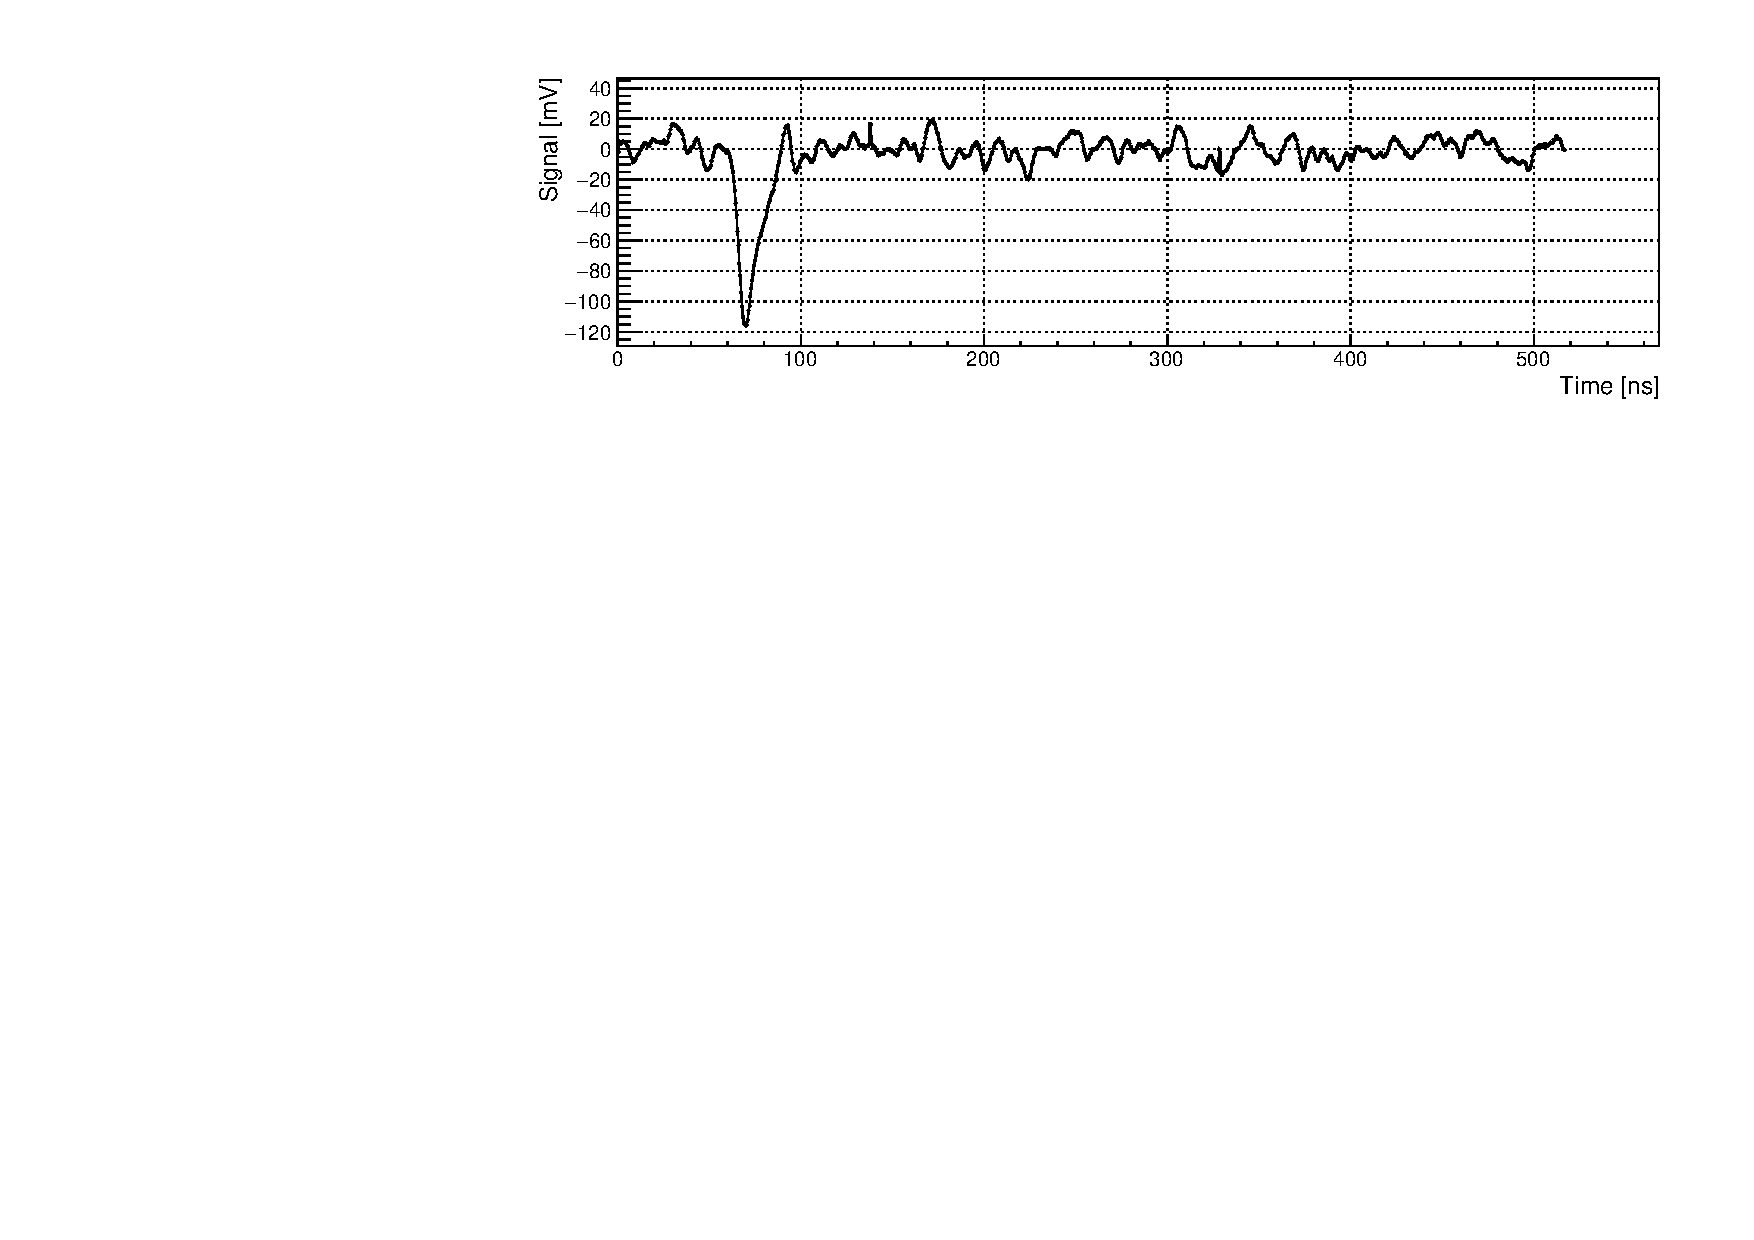
\includegraphics[angle=270, width=.73\textwidth]{SignalWaveform}\\
		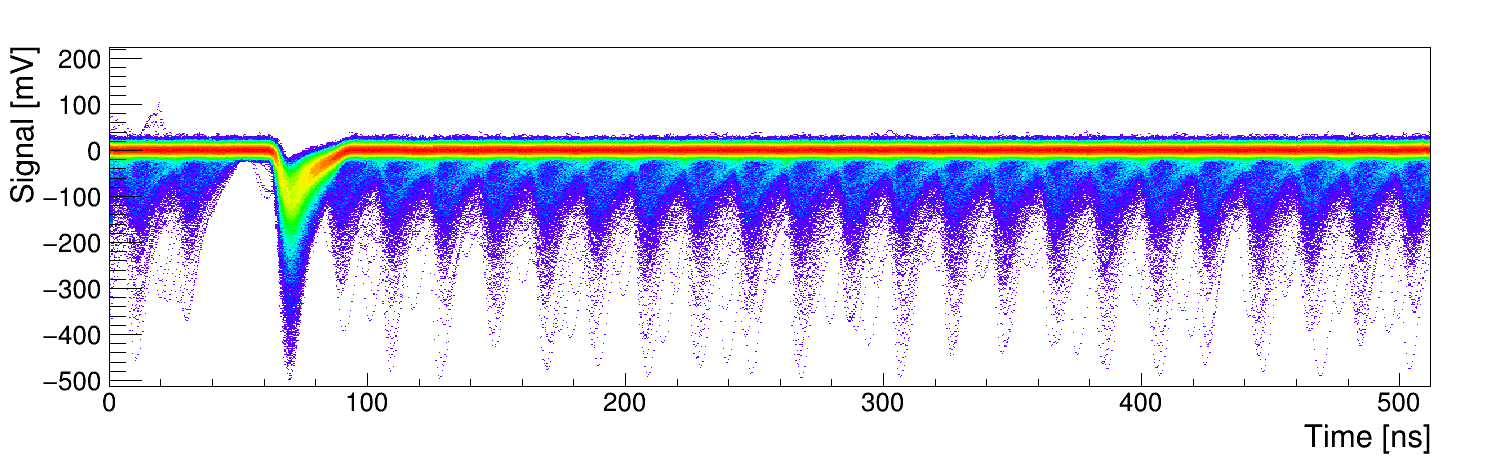
\includegraphics[width=.73\textwidth]{SignalWaveforms30000}
	\end{center}
	\begin{itemize}
		\item fast amplifier and good timing resolution \ra resolve bunch structure of PSI beam
		\item bunch spacing of \SI{19.8}{ns} clearly visible
	\end{itemize}
\end{frame}
% ============================ FRAME 4 ==========================================>
\begin{frame}{Results}

	\vspace*{-5pt}
	\begin{figure}[h]
		\begin{center}
			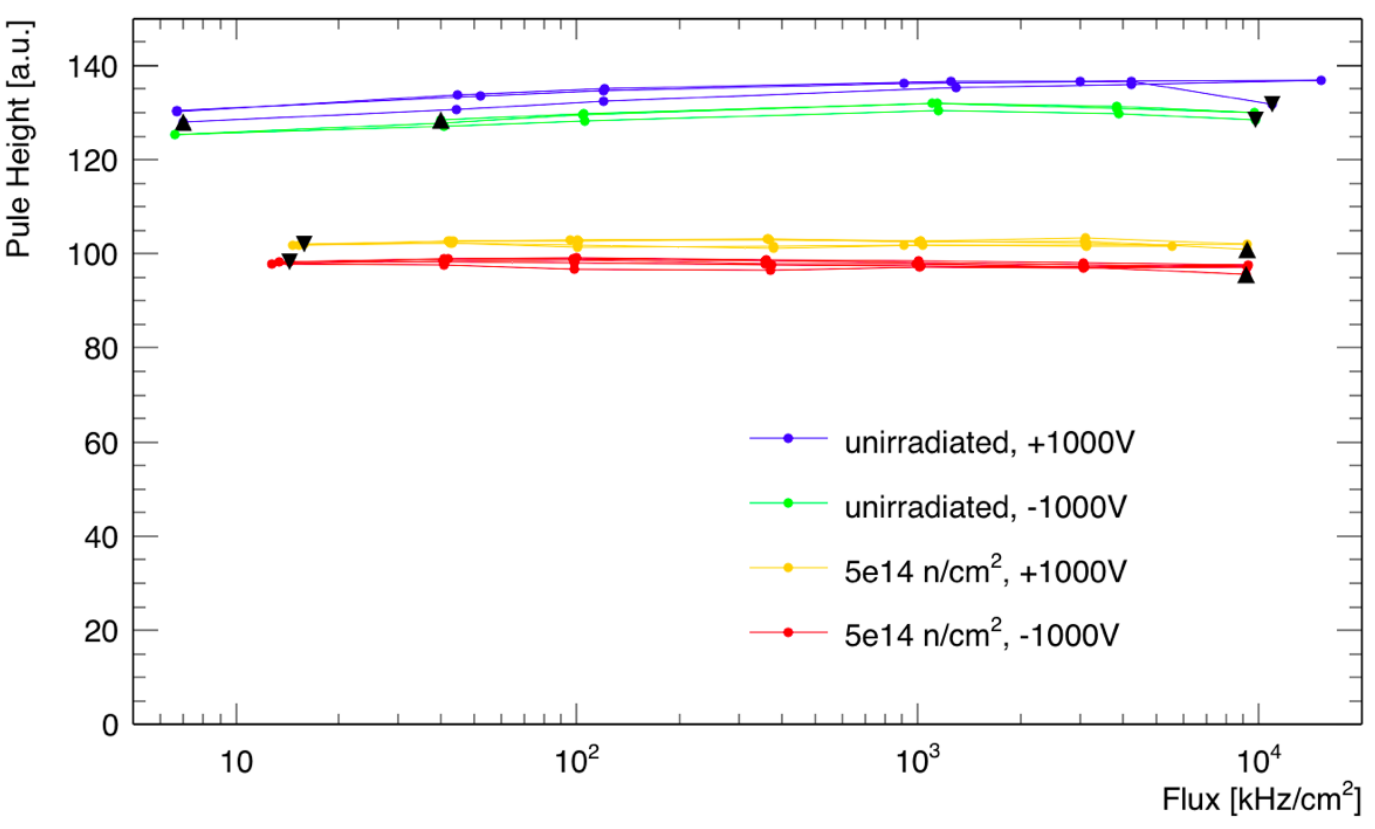
\includegraphics[width=.7\textwidth]{PadRates}
		\end{center}
	\end{figure}

	\begin{itemize}
		\item no rate dependence observed in pCVD diamonds up to \SI{10}{\mega\hertz\per cm^2}
		\item no absolute pulse height and noise calibration yet
		\item extending radiation doses to \SI{1e16}{n\per cm^2}
	\end{itemize}
\end{frame}


% ============= 5 =============
\section{3D Detector Development}
\subsection{3D Diamond Detectors}
\begin{frame}{Detector Concept}

	\vspace*{-5pt}
	\begin{itemize}
		\itemfill
		\item after large irradiation \ra all detector materials trap limited (mfp < \SI{75}{\micro\meter})
		\item \usebeamercolor[fg]{title} \textbf{keep drift distances smaller than mean free path}
	\end{itemize}

	\vspace*{-10pt}
	\begin{figure} 
		\begin{center}
			\begin{subfigure}{0.4\textwidth}  
				\centering 
				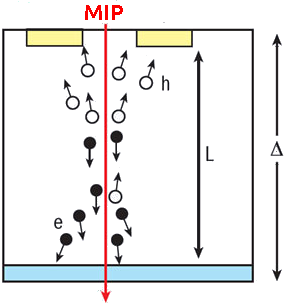
\includegraphics[height=.44\textheight]{PlanarConcept}
				\caption{planar detector}
			\end{subfigure}
			\begin{subfigure}{0.1\textwidth}  
				\centering 
				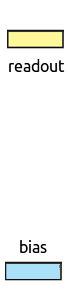
\includegraphics[height=.44\textheight]{LegendConcept}
				\vspace*{20pt}
			\end{subfigure}
			\begin{subfigure}{0.4\textwidth} 
				\centering 
				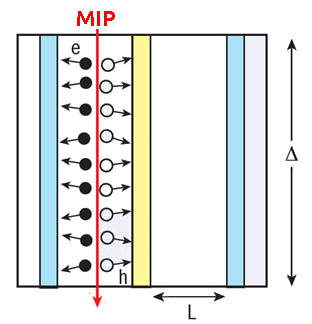
\includegraphics[height=.44\textheight]{3DConcept}
				\caption{3D detector} 	
			\end{subfigure} 
		\end{center}
	\end{figure}\vspace*{-15pt}
	
	\begin{itemize}
		\itemfill
		\item bias and readout electrode inside detector material
		\item same thickness $\Updelta$ \ra same amount of induced charge \ra shorter drift distance L
		\item electrode columns drilled with \SI{800}{\nano\meter} femtosecond laser 
		\item convert diamond into resistive mixture of carbon phases
	\end{itemize}

\end{frame}

% ============================ FRAME 2 ============================================
% \begin{frame}{3D Diamond Detectors}
% 
% 	\begin{itemize}
% 		\itemfill
% 		\item columns drilled with \SI{800}{\nano\meter} femtosecond laser 
% 		\item convert diamond into resistive mixture of carbon phases
% 	\end{itemize}
% 	
% 	\begin{figure}
% 		\centering 
% 		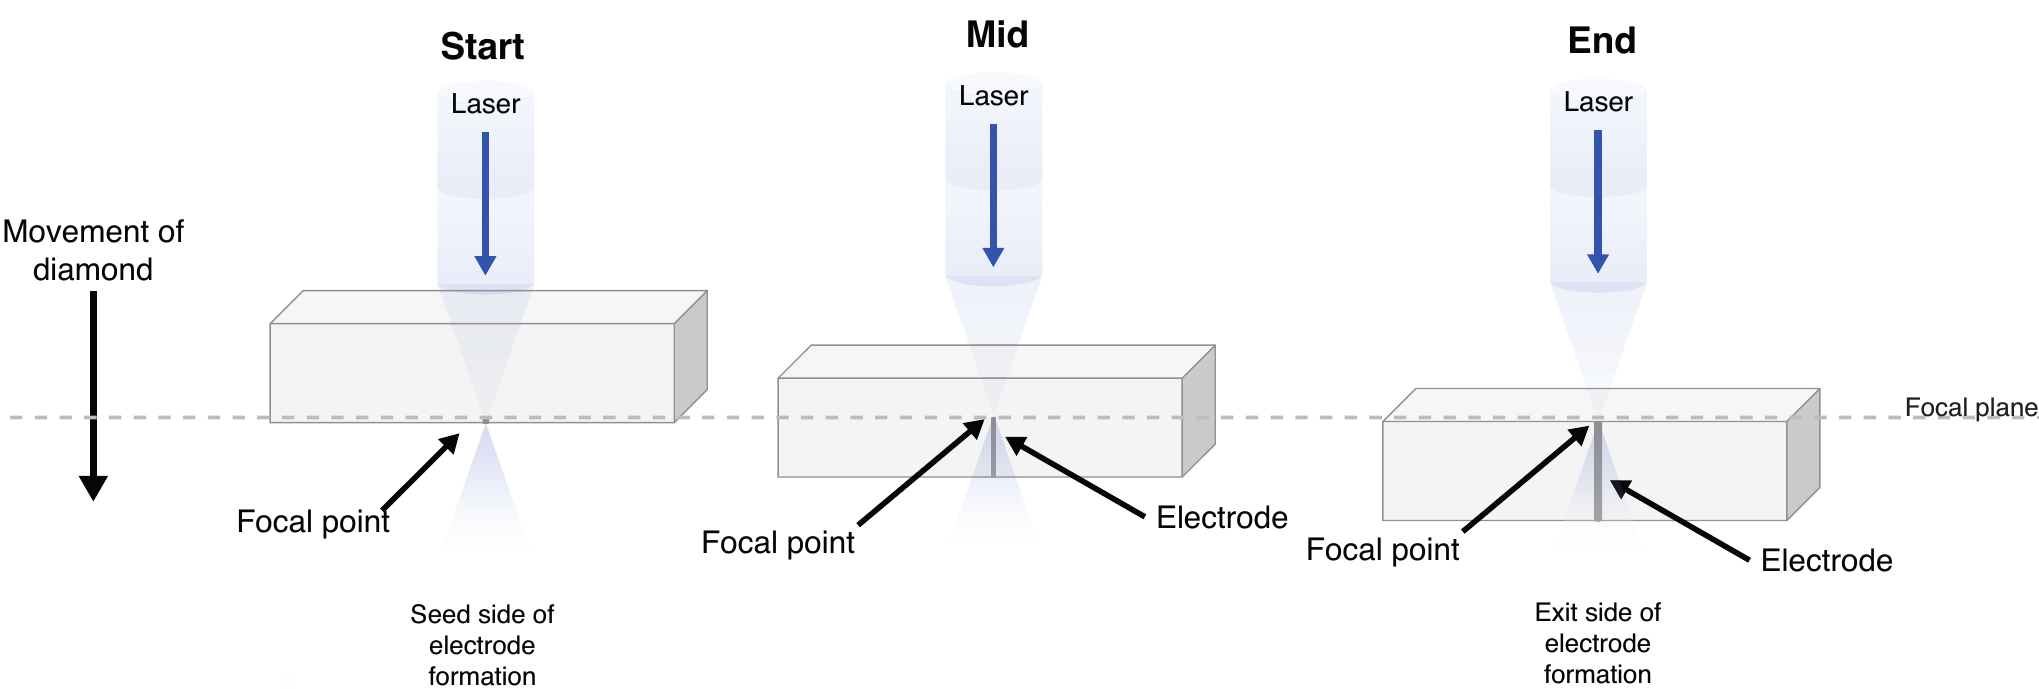
\includegraphics[width=.9\textwidth]{Fabrication}
% 	\end{figure}
% 	
% 	\begin{itemize}
% 		\itemfill
% 		\item 3 years ago: results of scCVD diamond detector
% 		\item 2 years ago: first 3D device in pCVD
% 		\item last year: first 3D pixel detector in pCVD diamond
% 	\end{itemize}
% 
% \end{frame}

% ============================ FRAME 3 ============================================
\begin{frame}{3D Multi Detector (2015)}

	\begin{itemize}
		\itemfill
		\item pCVD diamond with 3D, phantom and strip detector on single sensor
		\item 3D column efficiency of \SI{92}{\%}
		\item 3D cell size: \SI{150x150}{\micro\meter}
		\item signal read out as ganged cells
	\end{itemize}
	
	\begin{figure}
		\centering
		\begin{subfigure}{0.45\textwidth}  
			\centering 
			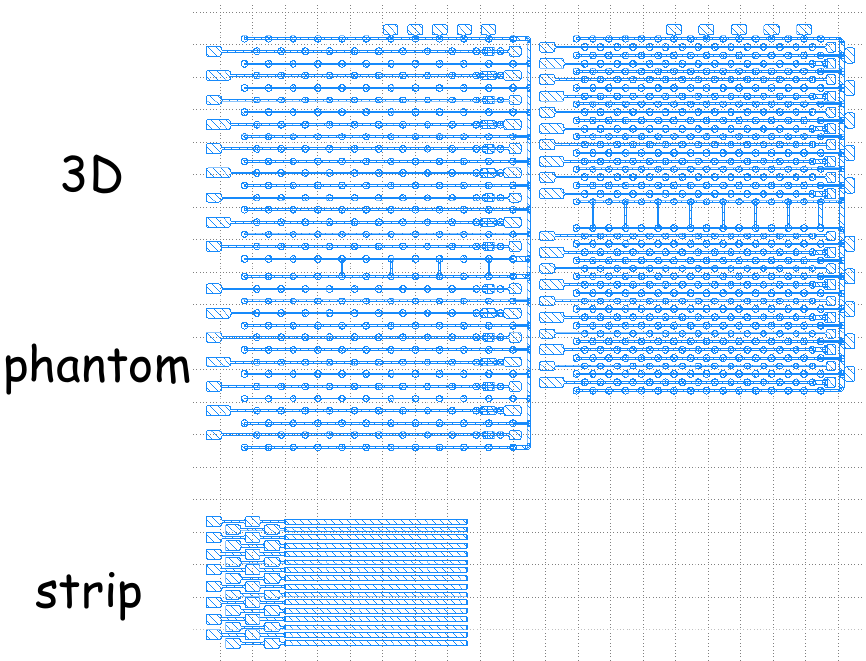
\includegraphics[height=.44\textheight]{3DMultiScheme}
			\caption{metalisation pattern}
		\end{subfigure}
		\begin{subfigure}{0.45\textwidth} 
			\centering 
			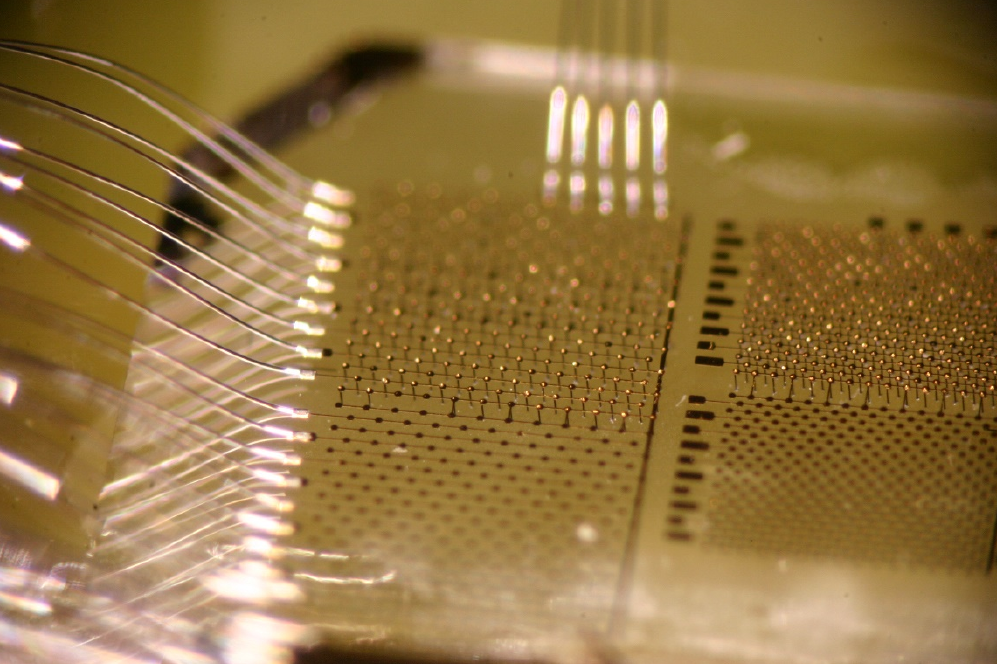
\includegraphics[height=.44\textheight]{3DMulti2}
			\caption{photograph}
		\end{subfigure}
	\end{figure}\vspace*{-15pt}

\end{frame}

% ============================ FRAME 4 ============================================
\begin{frame}{3D Multi - Signal Map}

	\begin{itemize}
		\itemfill
		\item square cells visible (9 broken cells)
		\item signals in 3D already bigger by eye
		\item phantom (no columns) \ra no pulse height
	\end{itemize}
	
	\begin{figure}
		\centering 
		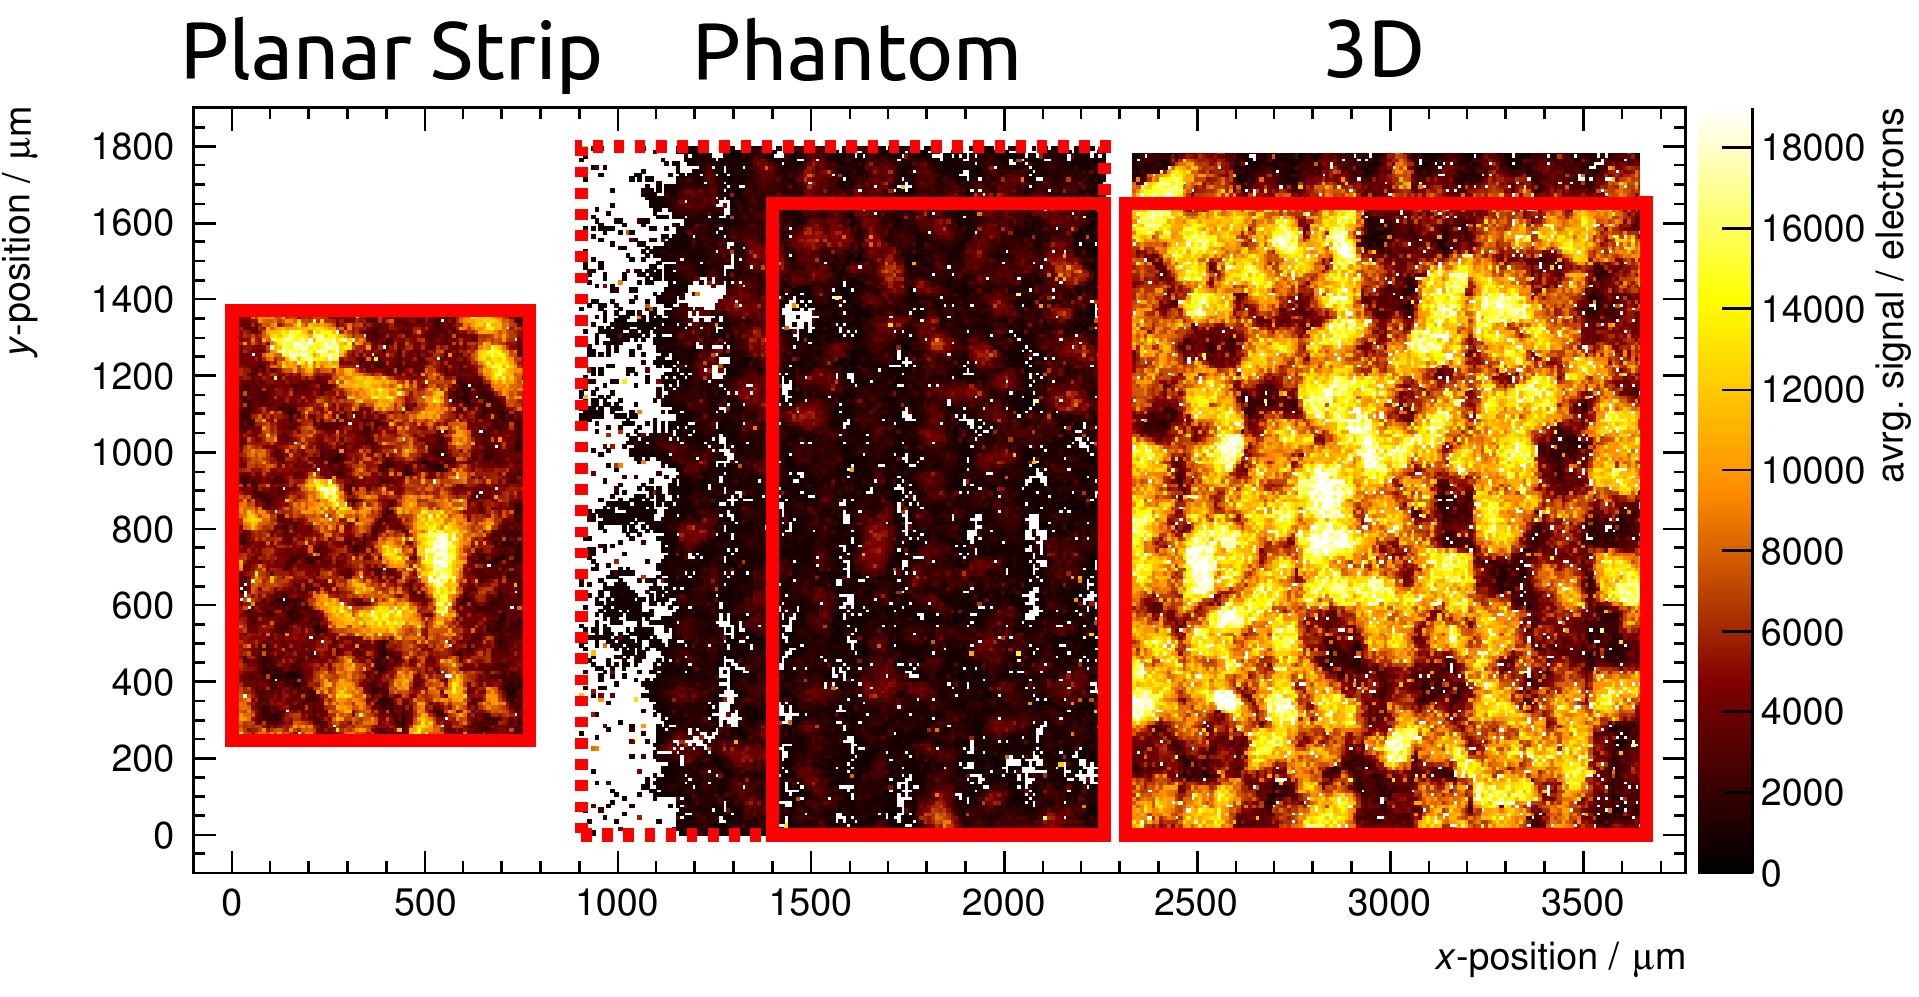
\includegraphics[height=.6\textheight]{3DMulti1}
	\end{figure}\vspace*{-10pt}

\end{frame}
% ============================ FRAME 5 ============================================
\begin{frame}{3D Multi - Result}

	\begin{itemize}
		\itemfill
		\item measured signals for diamond thickness \SI{500}{\micro\meter}:
	\end{itemize}
	
	\begin{table}
		\begin{tabular}[c]{c|c|c}
			\noalign{\hrule height 1pt}
			\rowcolor{title in head/foot.bg!70!white} 
			\multicolumn{1}{c|}{\textbf{Device}} & \multicolumn{1}{c|}{\textbf{Mean Charge [e]}} & \multicolumn{1}{c}{\textbf{ccd [$\upmu$m]}} \\\hline
			\rowcolor{date in head/foot.bg!30!white} 
			planar strip 	& $6900$ 	& $192$ 		\\\hline
			3D				& $13500$ 	& $350 - 375$* 	\\\hline
			\noalign{\hrule height 1pt}
		\end{tabular}
	\end{table}
	\begin{itemize}
		\itemfill
		\item *ccd$_{\z{eq}}$ - equivalent ccd to observe same charge in planar device
		\item \good{collect > \SI{75}{\%} charge in pCVD for the first time}
	\end{itemize}
	
	\begin{figure}
		\centering 
		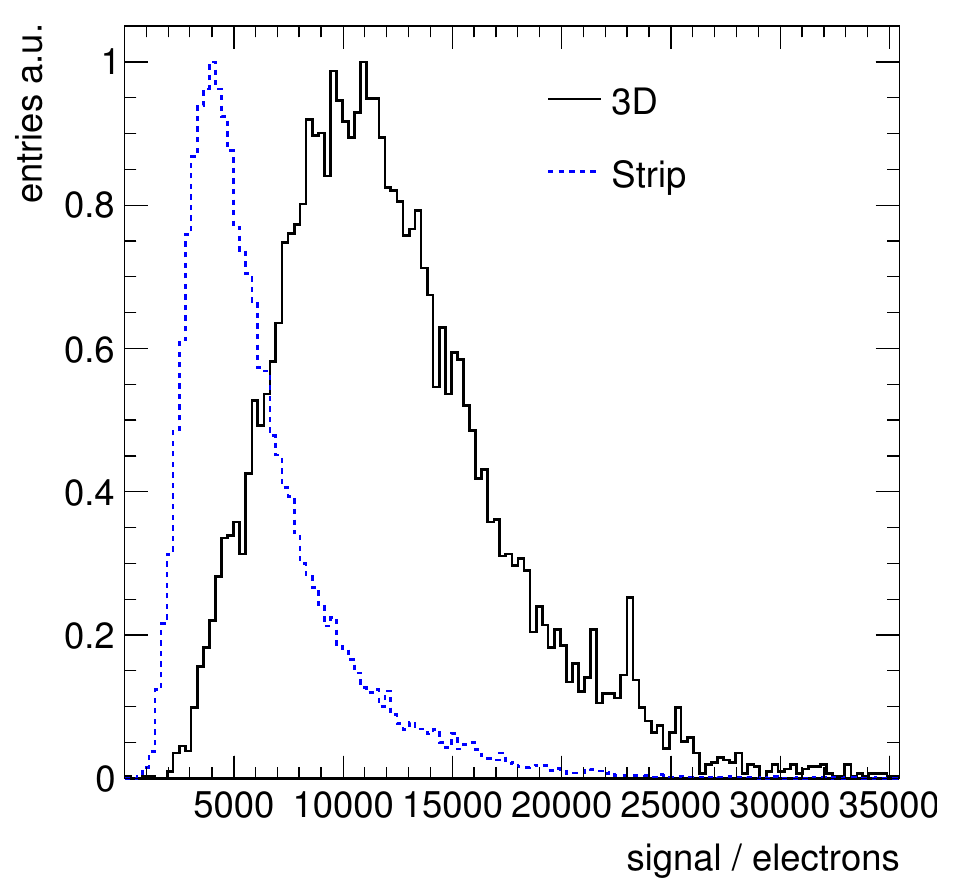
\includegraphics[height=.5\textheight]{3DMultiResult}
	\end{figure}\vspace*{-10pt}

\end{frame}
% ============================ FRAME 6 ============================================
\begin{frame}{Full 3D Detector (May/Sep 2016)}

	\begin{itemize}
		\itemfill
		\item 3 dramatic improvements compared to 3D Multi:
		\vspace*{3pt}
			\begin{itemize}
				\itemfill
				\item an order of magnitude more cells: from \SIrange{99}{1188}{}
				\item smaller cell size: \SI{100x100}{\micro\meter}
				\item higher column efficiency: from \SIrange{92}{99}{\%}
			\end{itemize}

	\end{itemize}
	
	\begin{figure}
		\centering
		\begin{subfigure}{0.45\textwidth}  
			\centering 
			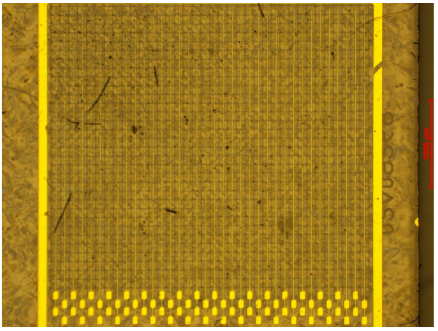
\includegraphics[height=.48\textheight]{3DFull1}
			\caption{readout side}
		\end{subfigure}
		\begin{subfigure}{0.45\textwidth} 
			\centering 
			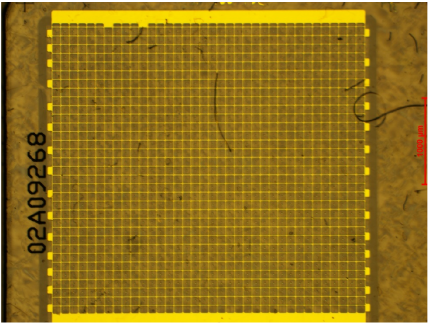
\includegraphics[height=.48\textheight]{3DFull2}
			\caption{bias side}
		\end{subfigure}
	\end{figure}\vspace*{-15pt}

\end{frame}
% ============================ FRAME 6 ============================================
\begin{frame}{Full 3D Preliminary Results}

	\begin{itemize}
		\itemfill
		\item analysis in progress
		\item device seems to perform well
		\item see charge in entire detector
		\item largest charge collection in pCVD yet
		\begin{itemize}
			\vspace*{1pt}
			\item \good{\SI{>85}{\%} over contiguous region}
		\end{itemize}
	\end{itemize}
	
	\vspace*{-5pt}
	\begin{figure}
		\centering
		\begin{subfigure}{0.45\textwidth}  
			\centering 
			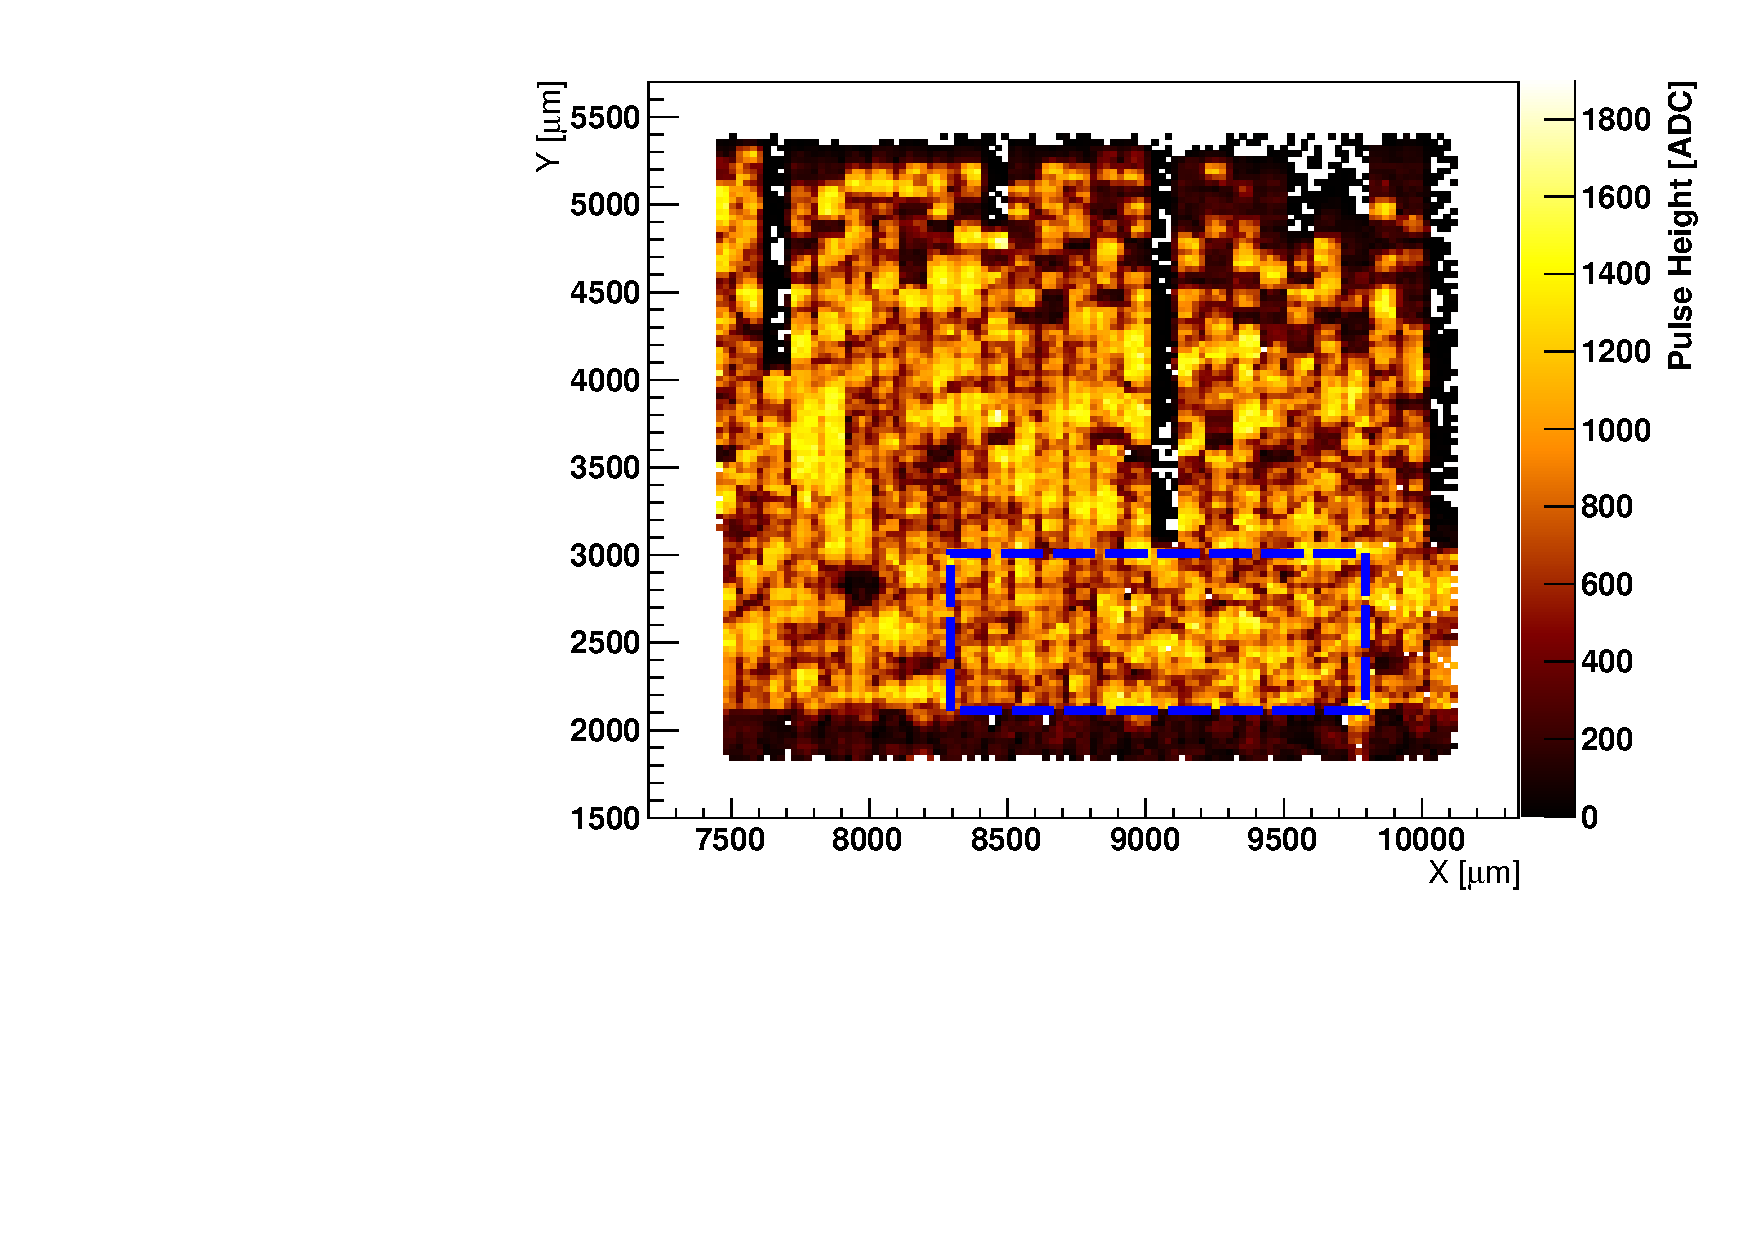
\includegraphics[width=.5\textheight, angle=-90]{3DFullCharge}
			\caption{charge map}
		\end{subfigure}
		\begin{subfigure}{0.45\textwidth} 
			\centering 
			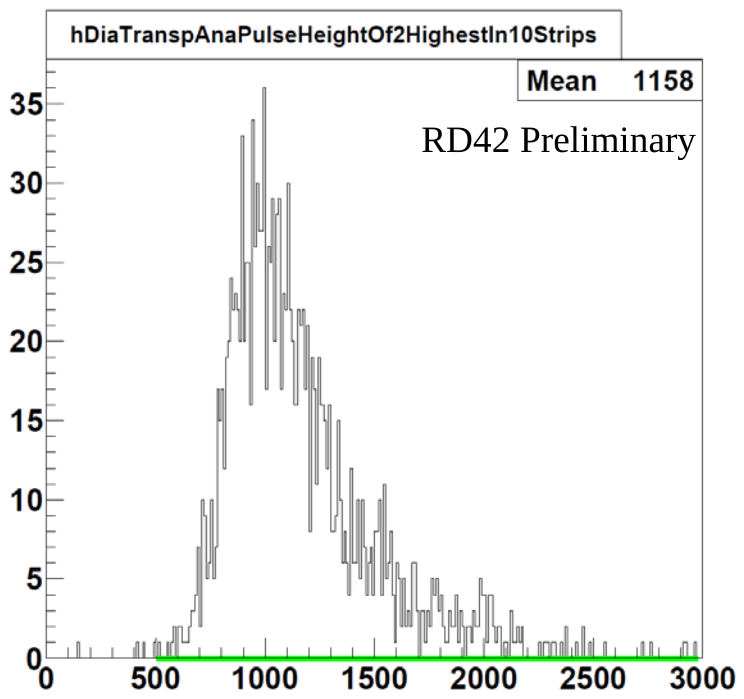
\includegraphics[width=.5\textheight, angle=-90]{3DFullDisto}
			\caption{charge distribution}
		\end{subfigure}
	\end{figure}\vspace*{-15pt}

\end{frame}

% ============================ FRAME 7 ============================================
\begin{frame}{3D Pixel Detector - Fabrication}

	\vspace*{-5pt}
	\begin{itemize}
		\itemfill
		\item cleaning and photo-lithography
		\item connect to bias and readout with surface metallisation
		\item bump and wire bonding
	\end{itemize}
	
	\begin{figure}
		\centering
		\begin{subfigure}{0.45\textwidth}  
			\centering 
			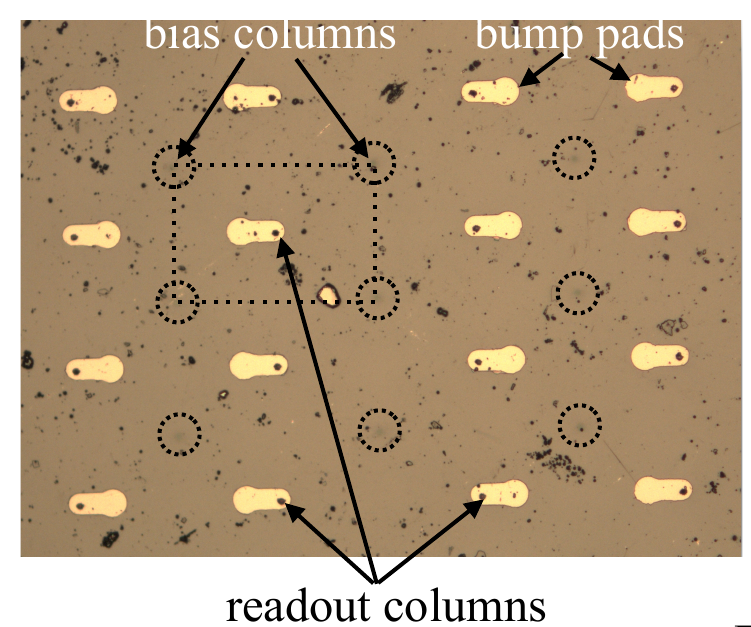
\includegraphics[height=.48\textheight]{BumpPads}
			\caption{pixel readout metalisation}
		\end{subfigure}
		\hspace*{10pt}
		\begin{subfigure}{0.45\textwidth} 
			\centering 
			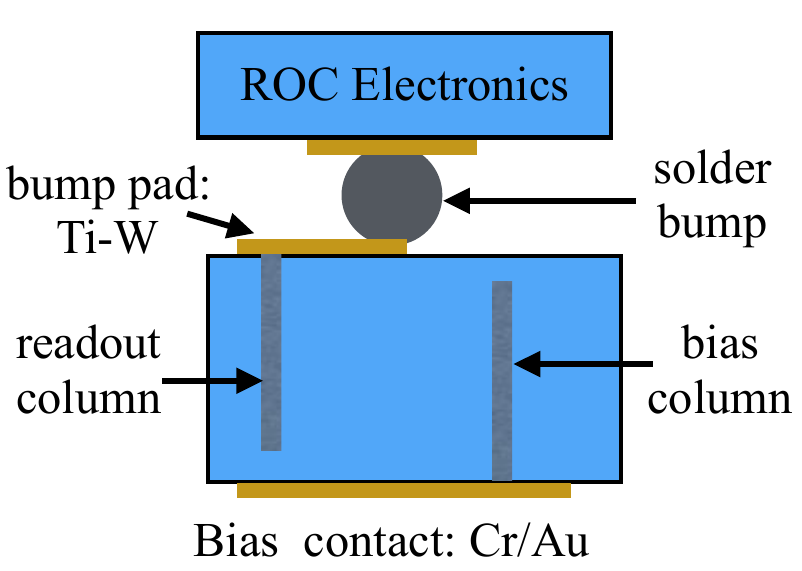
\includegraphics[height=.48\textheight]{FabFinalScheme}
			\caption{final scheme}
		\end{subfigure}
	\end{figure}\vspace*{-15pt}
 	
\end{frame}
% ============================ FRAME 7 ============================================
\begin{frame}{3D Pixel Detector}
	
	\begin{figure}
		\centering
		\begin{subfigure}{0.45\textwidth}  
			\centering 
			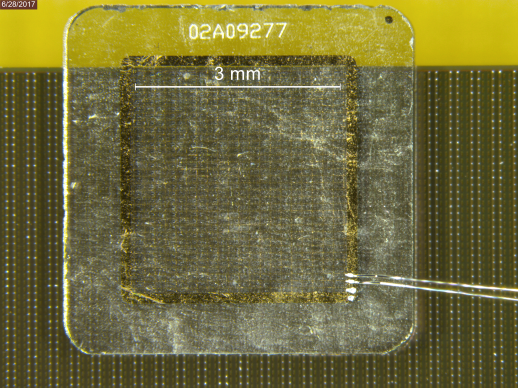
\includegraphics[height=.44\textheight]{3DFull}
			\caption{detector bonded on CMS-Pixel-Chip}
		\end{subfigure}
		\begin{subfigure}{0.45\textwidth} 
			\centering 
			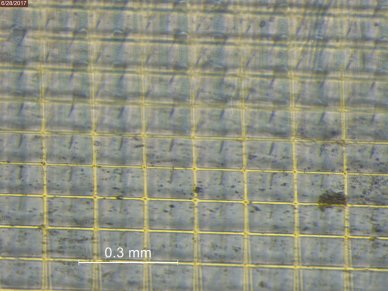
\includegraphics[height=.44\textheight]{3DCols}
			\caption{bias grid and R/O columns}
		\end{subfigure}
	\end{figure}

	\begin{itemize}
		\itemfill
		\item successful production of a working 3D pixel detector
	\end{itemize}
 	
\end{frame}
% ============================ FRAME 8 ============================================
\begin{frame}{3D Pixel Detector - Preliminary Results}

	\begin{minipage}{.4\textwidth}
		\hfill 3D Diamond Pixel\\
		\good{\hfill\ra\SI{98.5}{\%} Efficiency}
		
		\vspace*{20pt}
		\color{black}
		\begin{itemize}
			\color{black}
			\item efficiencies flat in time
			\item pixel threshold: \SI{1500}{e}
			\item lower efficiency in diamond probably due to due to low field regions
		\end{itemize}
		\vspace*{20pt}
		
		\hfill Planar Silicon Pixel (Ref)\\
		\good{\hfill\ra\SI{99.3}{\%} Efficiency}

	\end{minipage}
	\hspace*{2pt}
	\begin{minipage}{.56\textwidth}
		\begin{figure}[h]
			\centering
			\begin{subfigure}{0.45\textwidth}  
				\centering 
				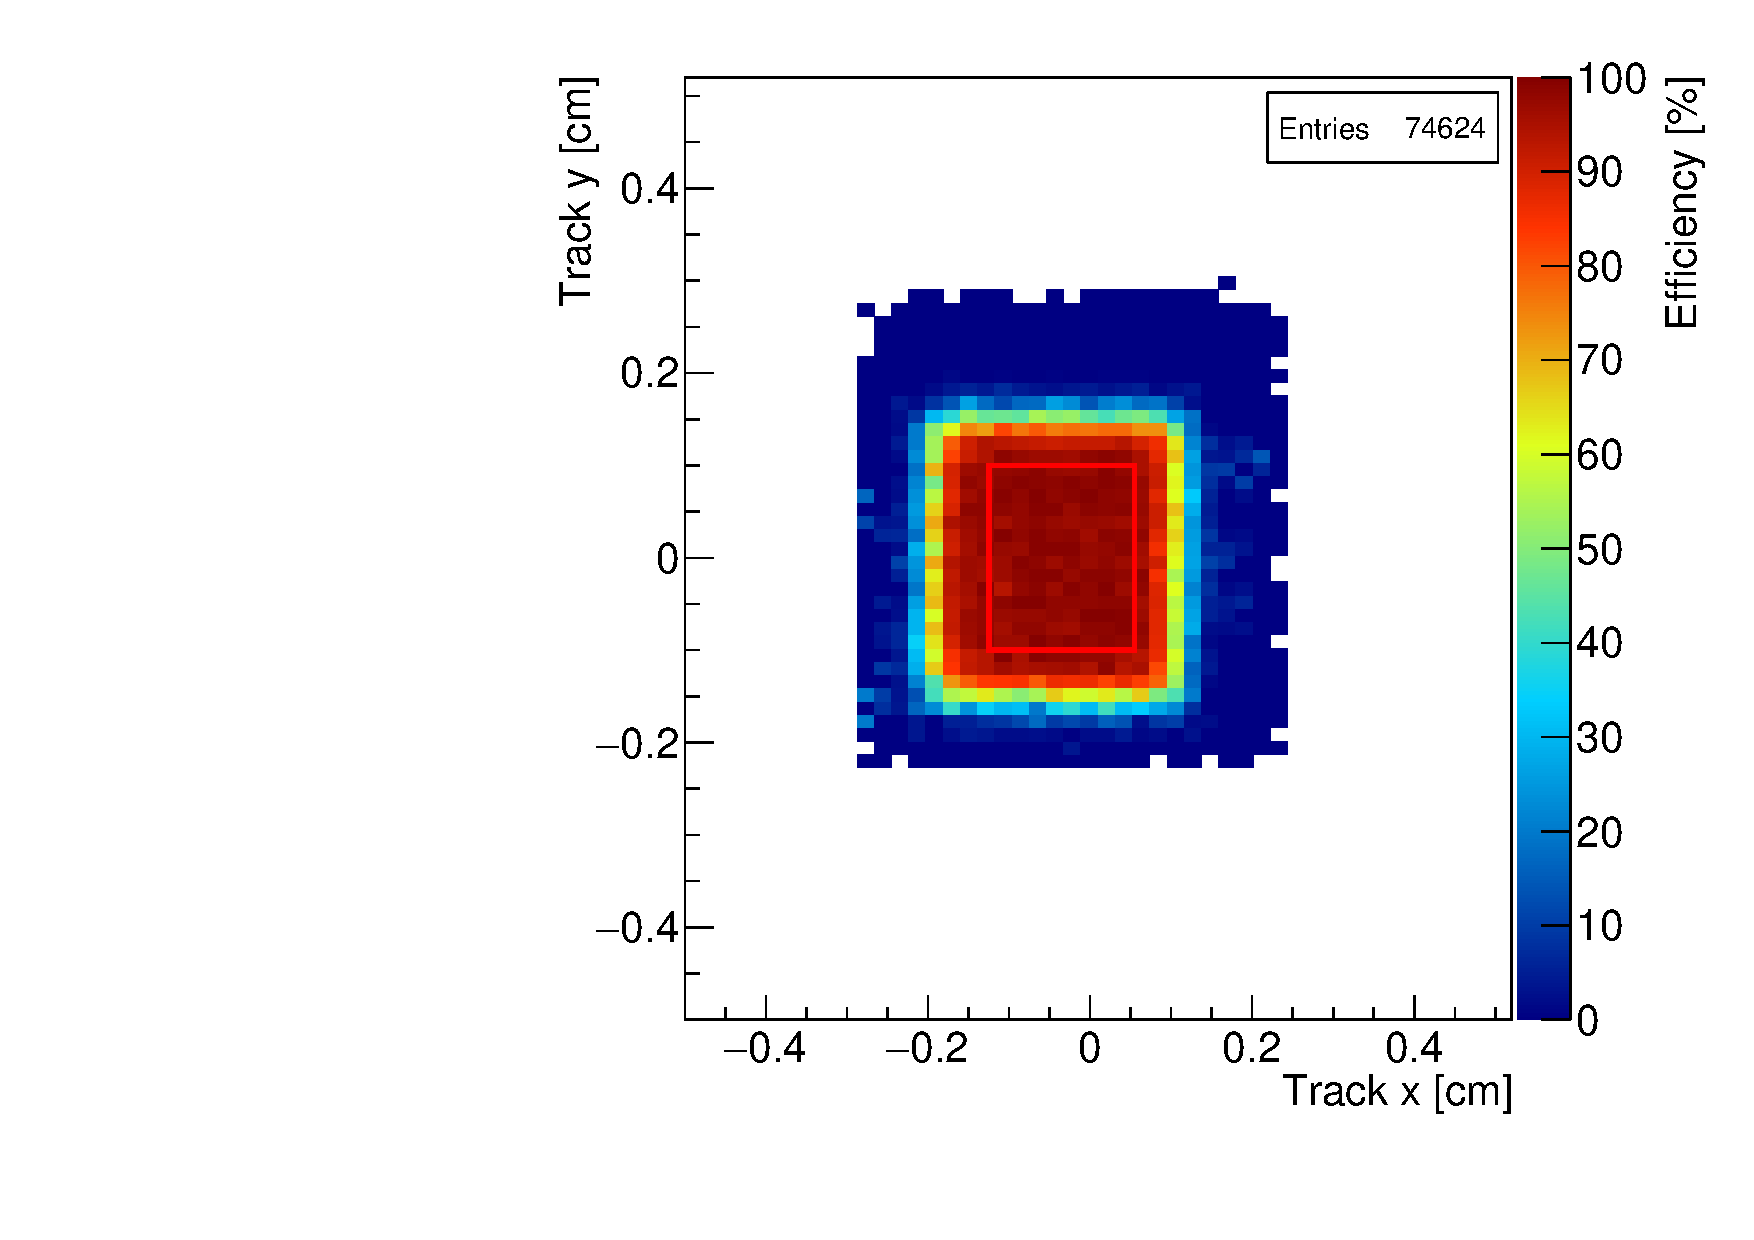
\includegraphics[width=.4\textheight, angle=-90]{EffMapDia}
			\end{subfigure}
			\begin{subfigure}{0.45\textwidth} 
				\centering 
				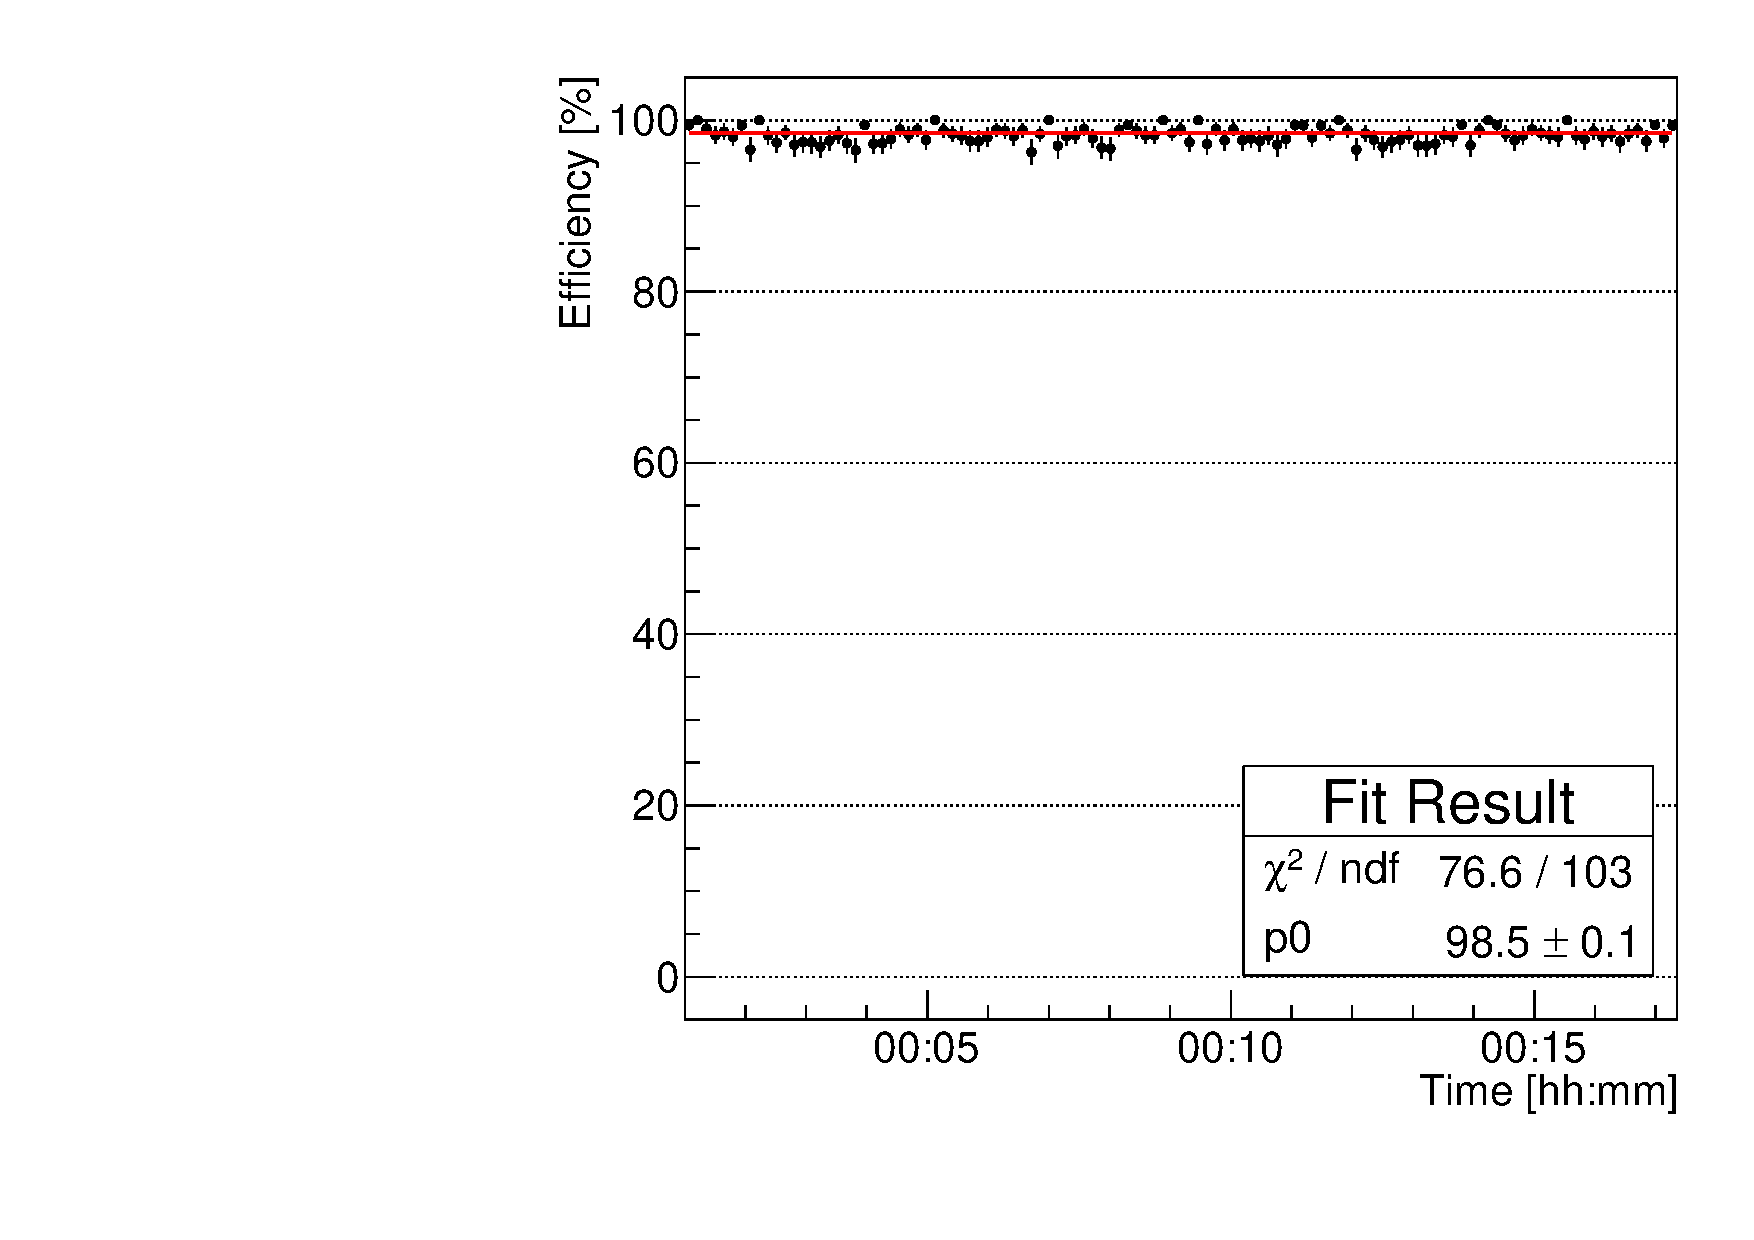
\includegraphics[width=.4\textheight, angle=-90]{HitEffDia}
			\end{subfigure}
			\begin{subfigure}{0.45\textwidth}  
				\centering 
				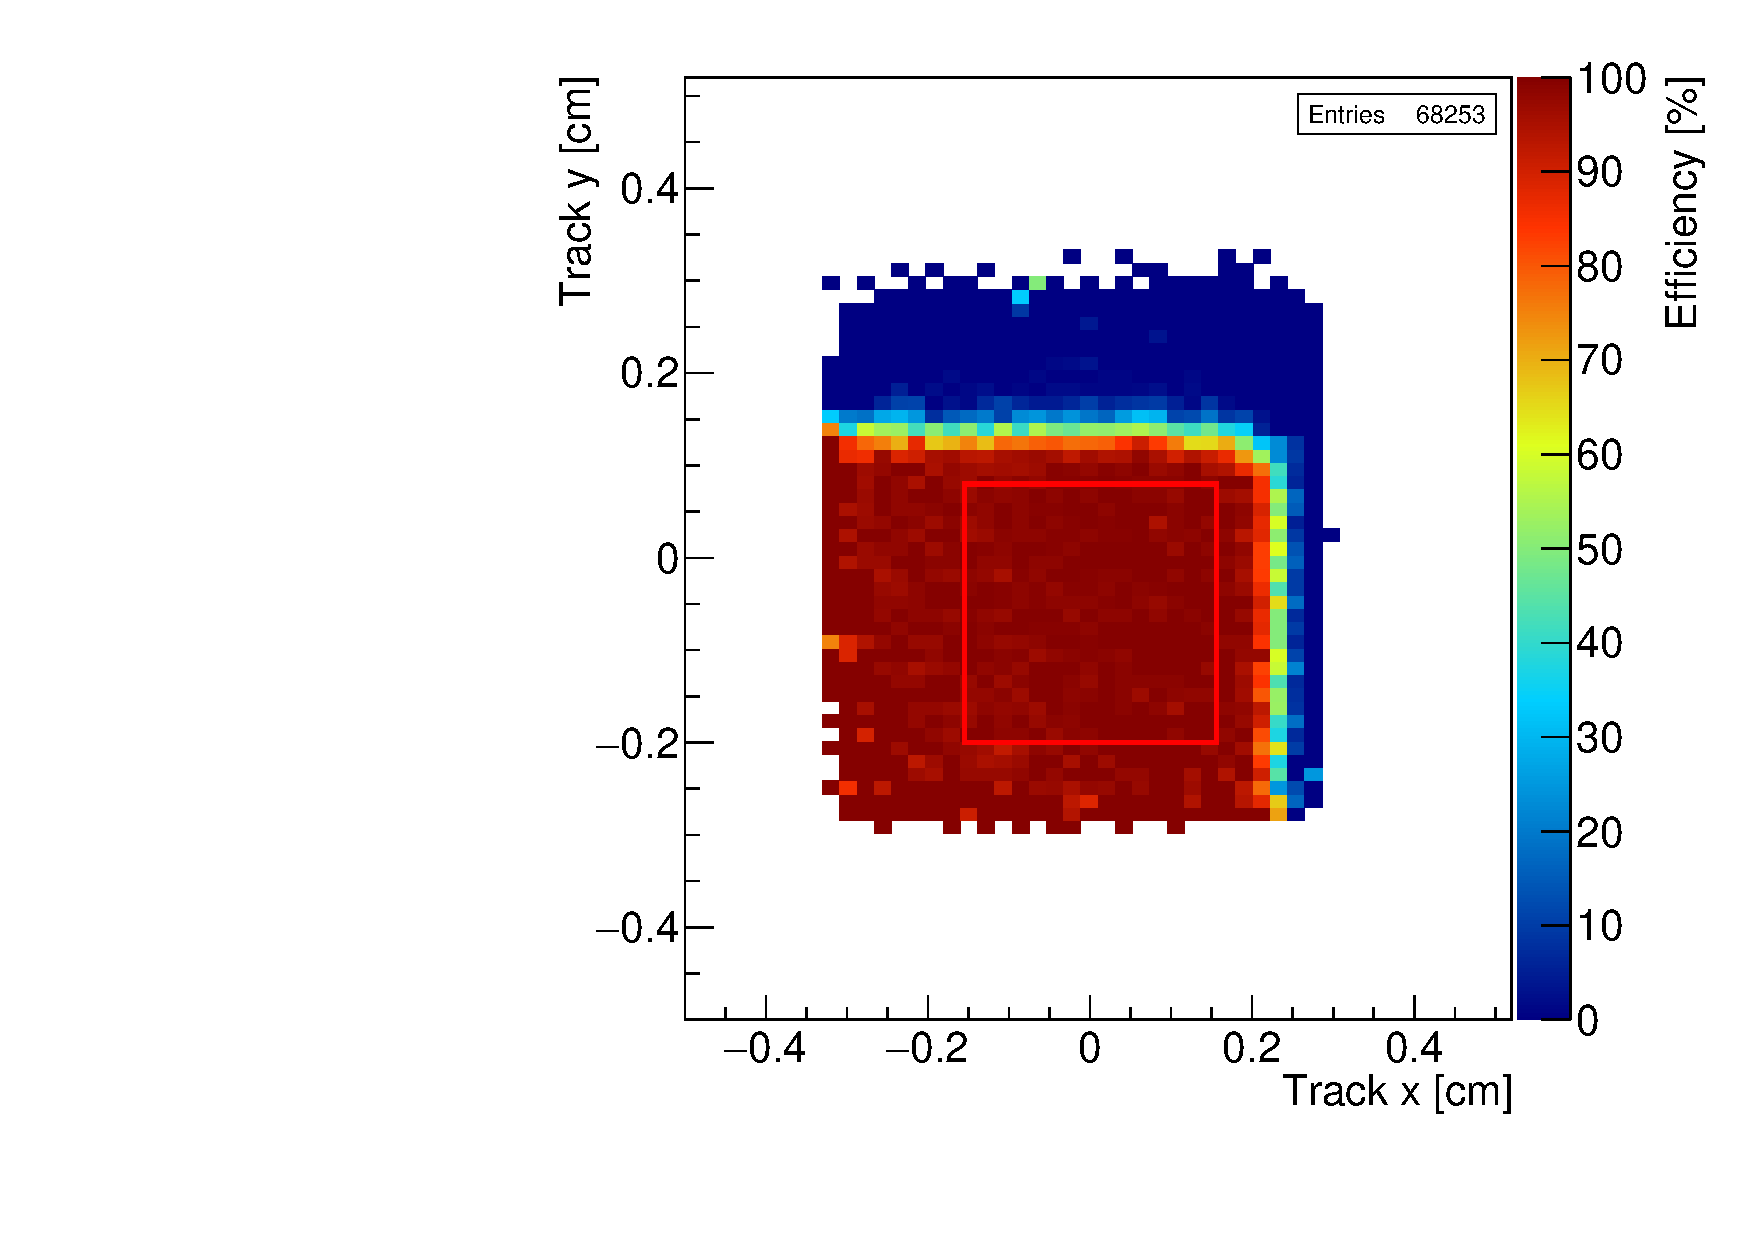
\includegraphics[width=.4\textheight, angle=-90]{EffMapSil}
				\caption{efficiency maps}
			\end{subfigure}
			\begin{subfigure}{0.45\textwidth} 
				\centering 
				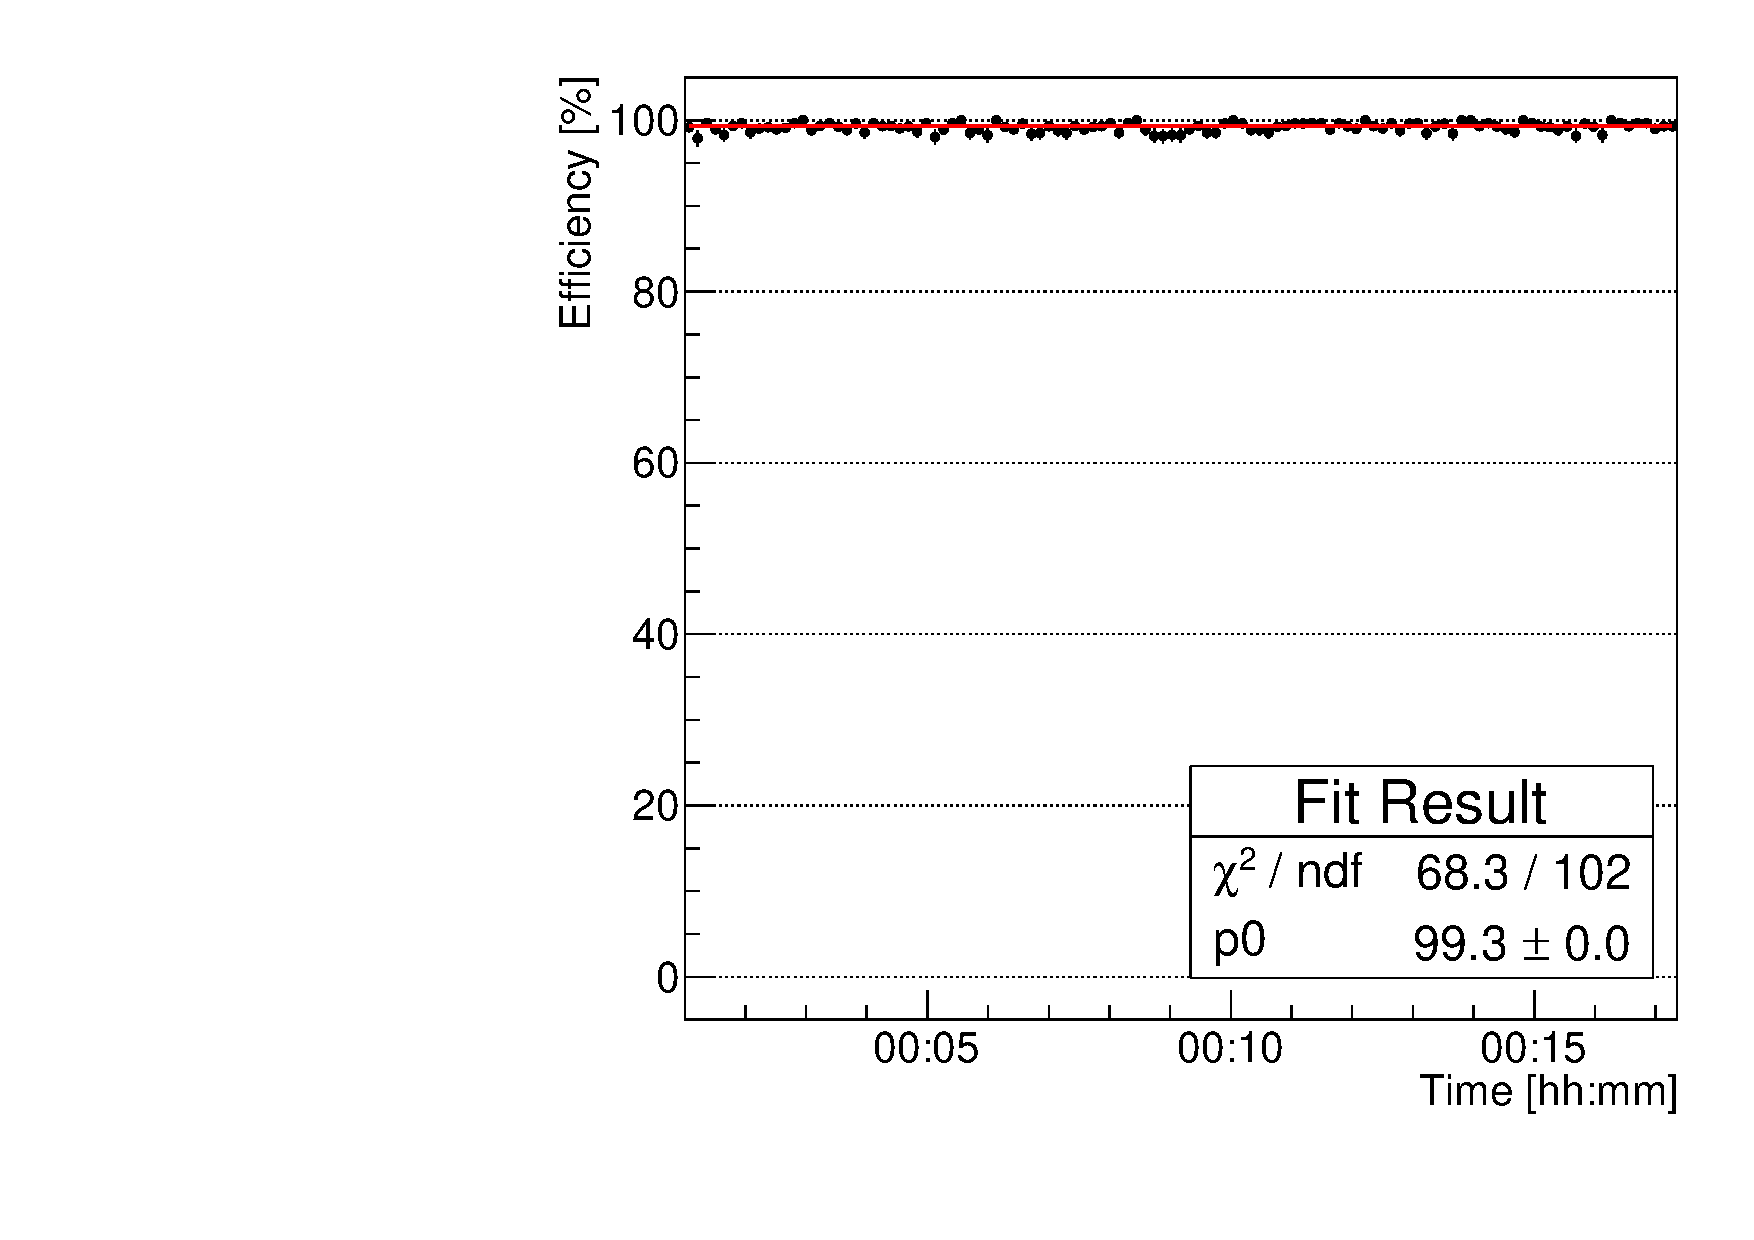
\includegraphics[width=.4\textheight, angle=-90]{HitEffSil}
				\caption{hit efficiencies}
			\end{subfigure}
		\end{figure}
	\end{minipage}
 	
\end{frame}
% ============================ FRAME 9 ============================================
\begin{frame}{3D Pixel Detector - New Design}

	\vspace*{-5pt}
	\begin{itemize}
		\itemfill
		\item currently producing \SI{3500}{cell} pixel prototype with \SI{50}{\micro\meter} pixel pitch
		\item two independent drillings (Oxford - complete, Manchester - in progress)
		\item bump bonding at Princeton (CMS) and IFAE (ATLAS)
		\item CMS device probably ready for August beam tests
	\end{itemize}\vspace*{-10pt}
	
	\begin{figure}
		\centering 
		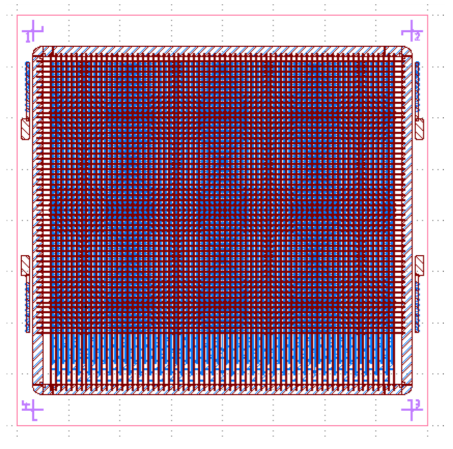
\includegraphics[height=.6\textheight]{3DNew}
	\end{figure}\vspace*{-15pt}
 	
\end{frame}




% ============= CONCLUSION =============
\section{Conclusion}
\begin{frame}{Conclusion}
	\begin{itemize}
		\itemfill
% 		\item closely working with manufacturers \ra increase diamond quality
		\item impact of diamonds in LHC is increasing
% 		\item ATLAS \& CMS BCM/BLM see collisions again
% 		\begin{itemize}
% 			\item abort, luminosity and background functionality in all LHC experiments
% 		\end{itemize}
		\item one of the first pixel projects started taking data:
		\begin{itemize}
			\item ATLAS DBM re-commissioned for \SI{13}{\tera\electronvolt} collisions
		\end{itemize}
		\item quantification and understanding of the rate effects in diamond
		\begin{itemize}
			\item pCVD shows no rate effect up to \SI{10}{\mega\hertz\per cm^2} 
			\item shown for fluence up to \SI{5e14}{n\per cm^2}
		\end{itemize}
		\item great progress in 3D detector prototypes
		\begin{itemize}
			\item 3D works in pCVD diamond; scale up and smaller cells also worked
		\end{itemize}
		\item production and successful test of 3D diamond pixel devices
		\begin{itemize}
			\item efficiency looks good; pulse height in progress
		\end{itemize}
	\end{itemize}
\end{frame}


% DOCUMENT END
\end{document}

